\documentclass[10pt, twocolumn, twoside, letterpaper]{IEEEtran}
\IEEEoverridecommandlockouts

\usepackage[activate={true, nocompatibility}, final, tracking=true, kerning=true, spacing=true, factor=1100, stretch=10, shrink=10]{microtype}
\linespread{0.9}

% \def\ps@IEEEtitlepagestyle{
%   \def\@oddfoot{\mycopyrightnotice}
%   \def\@evenfoot{}
% }
% \def\mycopyrightnotice{
%   {\footnotesize
%   \begin{minipage}{\textwidth}
%   \centering
%   978-1-7281-7693-2/20/\$31.00 \copyright2020 IEEE
%   \end{minipage}
%   }
% }

\ifCLASSINFOpdf
   \usepackage[pdftex]{graphicx}
\else
   \usepackage[dvips]{graphicx}
\fi

\ifCLASSOPTIONcompsoc
  \usepackage[caption=false, font=normalsize, labelfont=sf, textfont=sf]{subfig}
\else
  \usepackage[caption=false, font=footnotesize]{subfig}
\fi

\usepackage{amsmath}
\usepackage{bm}
\usepackage{amssymb}
%\usepackage{algorithm}
%\usepackage{algorithmic}
\usepackage[]{algorithm2e}
\DontPrintSemicolon
\usepackage{stfloats}
\usepackage{url}
\usepackage{siunitx}
\usepackage{fancyref}

\usepackage{geometry}
\geometry{letterpaper, top=0.7in, bottom=0.7in, left=0.65in, right=0.65in}

\usepackage[acronym, nomain]{glossaries}

% Define "long-s" key: 
\glsaddkey* {longs}% key 
{\glsentrylong{\glslabel}s}% default value 
{\glsentrylongs}% command analogous to \glsentrytext 
{\Glsentrylongs}% command analogous to \Glsentrytext 
{\glslongs}% command analogous to \glstext 
{\Glslongs}% command analogous to \Glstext 
{\GLSlongs}% command analogous to \GLStext

%% Define "short-s" key: 
\glsaddkey* {shorts}% key 
{\glsentryshort{\glslabel}s}% default value 
{\glsentryshorts}% command analogous to \glsentrytext 
{\Glsentryshorts}% command analogous to \Glsentrytext 
{\glsshorts}% command analogous to \glstext 
{\Glsshorts}% command analogous to \Glstext 
{\GLSshorts}% command analogous to \GLStext

\DeclareRobustCommand{\glss}[1]
{%
  \ifglsused{#1}{\glsshorts{#1}}{\glslongs{#1} (\glsshorts{#1})\glsunset{#1}}%
}

\DeclareRobustCommand{\Glss}[1]
{%
  \ifglsused{#1}{\Glsshorts{#1}}{\Glslongs{#1} (\glsshorts{#1})\glsunset{#1}}%
}

\newacronym{18F-FDG}{18F-FDG}{Fluorine-$18$ Fludeoxyglucose}
\newacronym{1D}{1D}{$1$-Dimensional}
\newacronym{2D}{2D}{$2$-Dimensional}
\newacronym{3D}{3D}{$3$-Dimensional}
\newacronym[longs={$3$-Dimensional Point Clouds}, shorts={3DPCs}]{3DPC}{3DPC}{$3$-Dimensional Point Cloud}
\newacronym{4D}{4D}{$4$-Dimensional}
% \newacronym{4DCT}{4DCT}{$4$-Dimensional Computed Tomography}
\newacronym{4DCT}{4DCT}{$4$D Computed Tomography}
\newacronym{AC}{AC}{Attenuation Corrected}
\newacronym{AD}{AD}{Affine Deformation}
\newacronym{AP}{AP}{Anterior Posterior}
\newacronym{ATP}{ATP}{Adenosine Triphosphate}
% \newacronym{AV-CCT}{AV-CCT}{Averaged CINE-Computed Tomography}
\newacronym{AV-CCT}{AV-CCT}{Averaged CINE-CT}
\newacronym{BE}{BE}{Bending Energy}
\newacronym{BFGS}{BFGS}{Broyden Fletcher Goldfarb Shanno}
\newacronym{CC}{CC}{Correlation Coefficient}
% \newacronym{CCT}{CCT}{CINE-Computed Tomography}
\newacronym{CCT}{CCT}{CINE-CT}
\newacronym{CG}{CG}{Conjugate Gradient}
\newacronym{COM}{COM}{Centre of Mass}
\newacronym[longs={Control Points}, shorts={CPs}]{CP}{CP}{Control Point}
\newacronym[longs={Control Point Grids}, shorts={CPGs}]{CPG}{CPG}{Control Point Grid}
\newacronym{CT}{CT}{Computed Tomography}
\newacronym{DDG}{DDG}{Data Driven Gating}
\newacronym{DD-PCA}{DD-PCA}{Data Driven Principal Component Analysis Surrogate Signal Extraction}
\newacronym{DD}{DD}{Data Driven}
\newacronym[longs={Deformation Vector Fields}, shorts={DVFs}]{DVF}{DVF}{Deformation Vector Field}
\newacronym{EANM}{EANM}{European Association of Nuclear Medicine}
\newacronym{EM}{EM}{Expectation Maximisation}
\newacronym{FDG}{FDG}{Fluorodeoxyglucose}
\newacronym{FFT}{FFT}{Fast Fourier Transform}
\newacronym[longs={Fields of View}, shorts={FOVs}]{FOV}{FOV}{Field of View}
\newacronym{FWHM}{FWHM}{Full Width at Half Maximum}
\newacronym{GAN}{GAN}{Generative Adversarial Networks}
\newacronym{GD}{GD}{Gradient Descent}
\newacronym{GE}{GE}{General Electric}
\newacronym{GT}{GT}{Ground Truth}
\newacronym{HU}{HU}{Hounsfield Unit}
\newacronym[longs={Image Registrations}, shorts={IRs}]{IR}{IR}{Image Registration}
\newacronym{KBq/mL}{KBq/mL}{Kilo Becquerel per Millilitre}
\newacronym{KeV}{KeV}{Kilo Electron Volt}
\newacronym{KRG}{KRG}{Kinetic Respiratory Gating}
\newacronym{KV}{KV}{Kilo Volt}
\newacronym{L-BFGS-B}{L-BFGS-B}{Low memory Broyden Fletcher Goldfarb Shanno Bounded}
\newacronym{L-BFGS}{L-BFGS}{Low memory Broyden Fletcher Goldfarb Shanno}
\newacronym[longs={Light Emitting Diodes}, shorts={LEDs}]{LED}{LED}{Light Emitting Diode}
\newacronym{LE}{LE}{Linear Energy}
\newacronym{LR}{LR}{Linear Regression}
\newacronym[longs={Lines of Response}, shorts={LORs}]{LOR}{LOR}{Line of Response}
\newacronym{MAE}{MAE}{Mean Absolute Error}
\newacronym{MAD}{MAD}{Median Absolute Difference}
\newacronym{MAPE}{MAPE}{Mean Absolute Percentage Error}
\newacronym{MBF}{MBF}{Myocardial Blood Flow}
\newacronym{MCIR}{MCIR}{Motion Compensated Image Reconstruction}
\newacronym[longs={Motion Compensated Images}, shorts={MCIs}]{MCI}{MCI}{Motion Compensated Image}
\newacronym{MC}{MC}{Motion Correction}
\newacronym{MIC}{MIC}{Medical Imaging Convention}
\newacronym{MI}{MI}{Mutual Information}
\newacronym{ML}{ML}{Maximum Likelihood}
\newacronym{MLAA}{MLAA}{Maximum Likelihood Reconstruction of Activity and Attenuation}
\newacronym{MLE}{MLE}{Maximum Likelihood Estimation}
\newacronym{MLEM}{MLEM}{Maximum Likelihood Expectation Maximisation}
\newacronym[longs={Motion Models}, shorts={MMs}]{MM}{MM}{Motion Model}
\newacronym{MPI}{MPI}{Myocardial Perfusion Imaging}
\newacronym{MR}{MR}{Magnetic Resonance}
\newacronym{MSc}{MSc}{Master of Science}
\newacronym{MSE}{MSE}{Mean Squared Error}
\newacronym[longs={Attenuation Maps}, shorts={Mu-Maps}]{Mu-Map}{Mu-Map}{Attenuation Map}
\newacronym{NAC}{NAC}{Non-Attenuation Corrected}
\newacronym{NMI}{NMI}{Normalised Mutual Information}
\newacronym{ND}{ND}{$n$-Dimensional}
\newacronym{NMC}{NMC}{Non-Motion Corrected}
\newacronym{NN}{NN}{Neural Network}
\newacronym{NRD}{NRD}{Non-Rigid Deformation}
\newacronym{NTOF}{NTOF}{Non-Time-of-Flight}
\newacronym{OSEM}{OSEM}{Ordered Subset Expectation Maximisation}
\newacronym[longs={Principal Components}, shorts={PCs}]{PC}{PC}{Principal Component}
\newacronym{PCA}{PCA}{Principal Component Analysis}
\newacronym{PCC}{PCC}{Pearson Correlation Coefficient}
\newacronym{PET}{PET}{Positron Emission Tomography}
\newacronym{PLL}{PLL}{Poisson Log Likelihood}
\newacronym{PSD}{PSD}{Power Spectral Density}
\newacronym{PSMA}{PSMA}{Prostate Specific Membrane Antigen}
\newacronym{RANSAC}{RANSAC}{Random Sample Consensus}
\newacronym{RCM}{RCM}{Respiratory Correspondence Model}
\newacronym{RD}{RD}{Rigid Deformation}
\newacronym{RDP}{RDP}{Relative Difference Prior}
\newacronym{RM}{RM}{Respiratory Motion}
\newacronym{RMC}{RMC}{Respiratory Motion Correction}
\newacronym{RMSE}{RMSE}{Root Mean Square Error}
\newacronym[longs={Regions of Interest}, shorts={ROIs}]{ROI}{ROI}{Region of Interest}
\newacronym{RPM}{RPM}{Real Time Position Management}
\newacronym{RTPM}{RTPM}{Real Time Position Management}
\newacronym{SAM}{SAM}{Spectral Analysis Method}
\newacronym{SGD}{SGD}{Stochastic Gradient Descent}
\newacronym{SI}{SI}{Superior Inferior}
\newacronym{SIRF}{SIRF}{Synergistic Image Reconstruction Framework}
\newacronym{SNR}{SNR}{Signal to Noise Ratio}
\newacronym[longs={Surrogate Signals}, shorts={SSs}]{SS}{SS}{Surrogate Signal}
\newacronym{SSD}{SSD}{Sum of Squared Differences}
\newacronym{STFT}{STFT}{Short-time Fourier transform}
\newacronym{STIR}{STIR}{Software for Tomographic Image Reconstruction}
\newacronym{SUV}{SUV}{Standard Uptake Value}
\newacronym{SVD}{SVD}{Singular Value Decomposition}
\newacronym{TOF}{TOF}{Time-of-Flight}
\newacronym{TPS}{TPS}{Thin Plate Spline}
\newacronym{XCAT}{XCAT}{$4$-Dimensional Extended Cardiac Torso}

% \glsunset{18F-FDG}
% \glsunset{1D}
% \glsunset{2D}
% \glsunset{3D}
% \glsunset{4D}
% \glsunset{4DCT}
% \glsunset{ATP}
% \glsunset{BFGS}
% \glsunset{CT}
% \glsunset{EANM}
% \glsunset{FDG}
% \glsunset{GE}
% \glsunset{L-BFGS-B}
% \glsunset{L-BFGS}
% \glsunset{LED}
% \glsunset{MIC}
% \glsunset{MLAA}
% \glsunset{MLEM}
% \glsunset{MR}
% \glsunset{MSc}
% \glsunset{Mu-Map}
% \glsunset{NTOF}
% \glsunset{OSEM}
% \glsunset{PCA}
% \glsunset{PET}
% \glsunset{RANSAC}
% \glsunset{RPM}
% \glsunset{RTPM}
% \glsunset{SIRF}
% \glsunset{STIR}
% \glsunset{SUV}
% \glsunset{TOF}
% \glsunset{XCAT}


\usepackage[style=ieee, doi=false, isbn=false, url=false, maxbibnames=1, minbibnames=1, maxcitenames=1, mincitenames=1, backend=biber, defernumbers=false]{biblatex}
\addbibresource{./bibtex/bib/Biblio.bib}

\AtEveryBibitem{\clearfield{month}}
\AtEveryBibitem{\clearfield{day}}
\AtEveryBibitem{\clearfield{volume}}
\AtEveryBibitem{\clearfield{issue}}
\AtEveryBibitem{\clearfield{pages}}
\AtEveryBibitem{\clearfield{number}}
\AtEveryBibitem{\clearfield{title}}
\AtEveryBibitem{\clearfield{isbn}}
\AtEveryBibitem{\clearfield{keywords}}
\AtEveryBibitem{\clearfield{issn}}
\AtEveryBibitem{\clearfield{journal}}

\begin{document}

\title{
    \vspace{-0.5cm}

    Data Driven Surrogate Signal Extraction for Dynamic PET using Selective PCA
}

\pagestyle{plain}
\pagenumbering{gobble}

\author{
    % \vspace{-0.3cm}
    
    \IEEEauthorblockN{
        Alexander~C.~Whitehead~\IEEEauthorrefmark{1}~\IEEEauthorrefmark{2},
        Kuan-Hao~Su~\IEEEauthorrefmark{3},
        Elise~C.~Emond~\IEEEauthorrefmark{1},
        Ander~Biguri~\IEEEauthorrefmark{1},
        Maria~Machado~\IEEEauthorrefmark{1},
        Joanna~C.~Porter~\IEEEauthorrefmark{4},
        Helen~Garthwaite~\IEEEauthorrefmark{4},
        Scott~D.~Wollenweber~\IEEEauthorrefmark{3},
        Charles~W.~Stearns~\IEEEauthorrefmark{3},
        Brian~F.~Hutton~\IEEEauthorrefmark{1},
        Jamie~R.~McClelland~\IEEEauthorrefmark{2} and
        Kris~Thielemans~\IEEEauthorrefmark{1}~\IEEEauthorrefmark{2}
    }
        
    \IEEEauthorblockA{
        \IEEEauthorrefmark{1}
        \textit{Institute of Nuclear Medicine, University College London, UK}
    }
    \IEEEauthorblockA{
        \IEEEauthorrefmark{2}
        \textit{Centre for Medical Image Computing, University College London, UK}
    }
    \IEEEauthorblockA{
        \IEEEauthorrefmark{3}
        \textit{Molecular Imaging and Computed Tomography Engineering, GE Healthcare, USA}
    }
    \IEEEauthorblockA{
        \IEEEauthorrefmark{4}
        \textit{Centre for Respiratory Medicine, University College London, London, UK}
        \vspace{-0.5cm}
    }

    \thanks{This research was supported by GE Healthcare, the NIHR UCLH Biomedical Research Centre and the UCL EPSRC Centre for Doctoral Training in Intelligent, Integrated Imaging in Healthcare (i4health) grant (EP/L016478/1).}
    \thanks{The software used was partly produced by the Computational Collaborative Project on Synergistic Biomedical Imaging, CCP SyneRBI, UK EPSRC grant (EP/T026693/1).}
    \thanks{Jamie~R.~McClelland is supported by a Cancer Research UK Centres Network Accelerator Award grant (A21993) to the ART-NET consortium and a CRUK Multi-disciplinary grant (CRC 521).}
    \thanks{(contact: \texttt{alexander.whitehead.18@ucl.ac.uk}).}
}

\maketitle
\IEEEpeerreviewmaketitle

\begin{abstract}
    Respiratory motion correction is beneficial in positron emission tomography. Methods of motion correction include gated reconstruction, where the acquisition is binned based on a respiratory trace. To acquire these respiratory traces an external device like the Real Time Position Management system or a data driven method such as principal component analysis can be used. Data driven methods have the advantage that they are non-invasive and can be performed post-acquisition. However, data driven methods have the disadvantage that they are adversely affected by the tracer kinetics of a dynamic acquisition. This work seeks to evaluate several adaptions of the principal component analysis method through which it can be used with dynamic data. The methods explored in this work include using a moving window, extrapolation of the principal component from later time frames to earlier time frames as well as a method to select and combine multiple respiratory components. The respiratory traces acquired were evaluated by calculating their correlation with a Real Time Position Management surrogate signal and also by performing and comparing gated reconstructions using the traces. The results indicate that all methods produce better surrogate signals than when applying static principle component analysis to dynamic data. extrapolating a 'late' principal component produced a more promising result than using a moving window and selecting and combining components held benefits for all methods. Future research includes using the extracted respiratory signals in more complex motion correction algorithms for dynamic PET.
\end{abstract}

\vspace{-0.5cm}

\vspace{2cm}
\section{INTRODUCTION} \label{sec:introduction}
    \IEEEPARstart{R}{espiratory} motion reduces image resolution by introducing blurring and mis-alignment artefacts~\cite{Nehmeh2008a}. Methods of \gls{MC} include gated reconstruction; bin the acquisition based on a \gls{SS}. This \gls{SS} is a respiratory trace which reflects the position of the patient in the respiratory cycle over time~\cite{Kesner2010AMethods, Kesner2013GatingPET}. Methods to determine the \gls{SS} include those which use an external device, for instance, the \gls{RPM}~\cite{Bettinardi2013Motion-trackingPET/CT}. A disadvantage of such methods are that they require the use of additional equipment, and a change to clinical practice. Thus, data driven methods to extract the \gls{SS} have become an alternative for static \acrshort{PET} data. However, current data driven methods are adversely affected by the radiotracer kinetics of a dynamic \acrshort{PET} acquisition; where the tracer is injected after the beginning of the scan. As an example, methods that use dimensionality reduction (such as \acrshort{PCA}~\cite{Thielemans2011, Bertolli2018Data-DrivenTomography}) are hampered by the fact that at the start of the scan, rapid redistribution of the radiotracer causes more variance in the data, than the respiratory motion.
    
    Previously, work was performed to extend \gls{SAM} to be robust to radiotracer kinetics. This work proposed the use of \gls{STFT}, to generate masks for \gls{SAM}. This was called \gls{KRG}~\cite{Schleyer2014}. \gls{STFT} operates by splitting the data into time windows, and doing a \acrlong{FFT} on them independently. This could be approximated by windowing the data first, and then performing \gls{SAM}.
    
    The aim of this work is to propose several adaptions of the \acrshort{PCA} method, through which it can be used with dynamic \acrshort{PET} data, and compare their performance with a method based on \gls{KRG}. The methods explored in this work include; the use of a moving window, re-use of the \glss{PC} from a later time point to estimate the \gls{SS} from earlier time points, and the automatic selection and combination of multiple \glss{PC}.

% \vspace{-0.5cm}
    
\section{METHODS} \label{sec:methods}
    \subsection{Data Acquisition} \label{sec:data_acquisition}
        Data was acquired from a research study with patients suffering from idiopathic pulmonary fibrosis. $21$ dynamic \acrshort{18F-FDG} \acrshort{PET} acquisitions, with a \acrlong{FOV} covering the upper lung and heart, were acquired on a \acrshort{GE} Discovery $710$~\cite{Oh2019OptimalTreatment, Emond2020EffectReconstruction}. \glss{SS} were acquired in parallel using the \gls{RPM}.
    
    % \vspace{-0.5cm}
        
    \subsection{Data Preparation} \label{sec:data_preparation}
        \gls{TOF} data were unlisted into low spatial resolution sinograms, each with a time frame duration of \SI{500}{\milli\second}, using the \acrshort{GE} PetToolbox, resulting in sinograms with dimensions $95\times16\times47\times11$ (radial positions$\times$angles$\times$transaxial plane$\times$\gls{TOF}).
        
        Data was pre-processed, first by applying a Freeman-Tukey transformation~\cite{Freeman1950TransformationsRoot}, before then applying a Yeo-Johnson power transformation~\cite{Yeo2000ASymmetry}. This is in order to attempt to transform the Poisson distributed data to be more Gaussian-like. The resultant sinograms are further spatially downsampled.
        
        \acrshort{PCA} was applied to the \gls{TOF} data~\cite{Bertolli2017DataData}.
    
    % \vspace{-0.5cm}
        
    \subsection{Moving Window} \label{sec:moving_window}
        \begin{figure}
            % \vspace{-0.5cm}
            
            \centering
            
            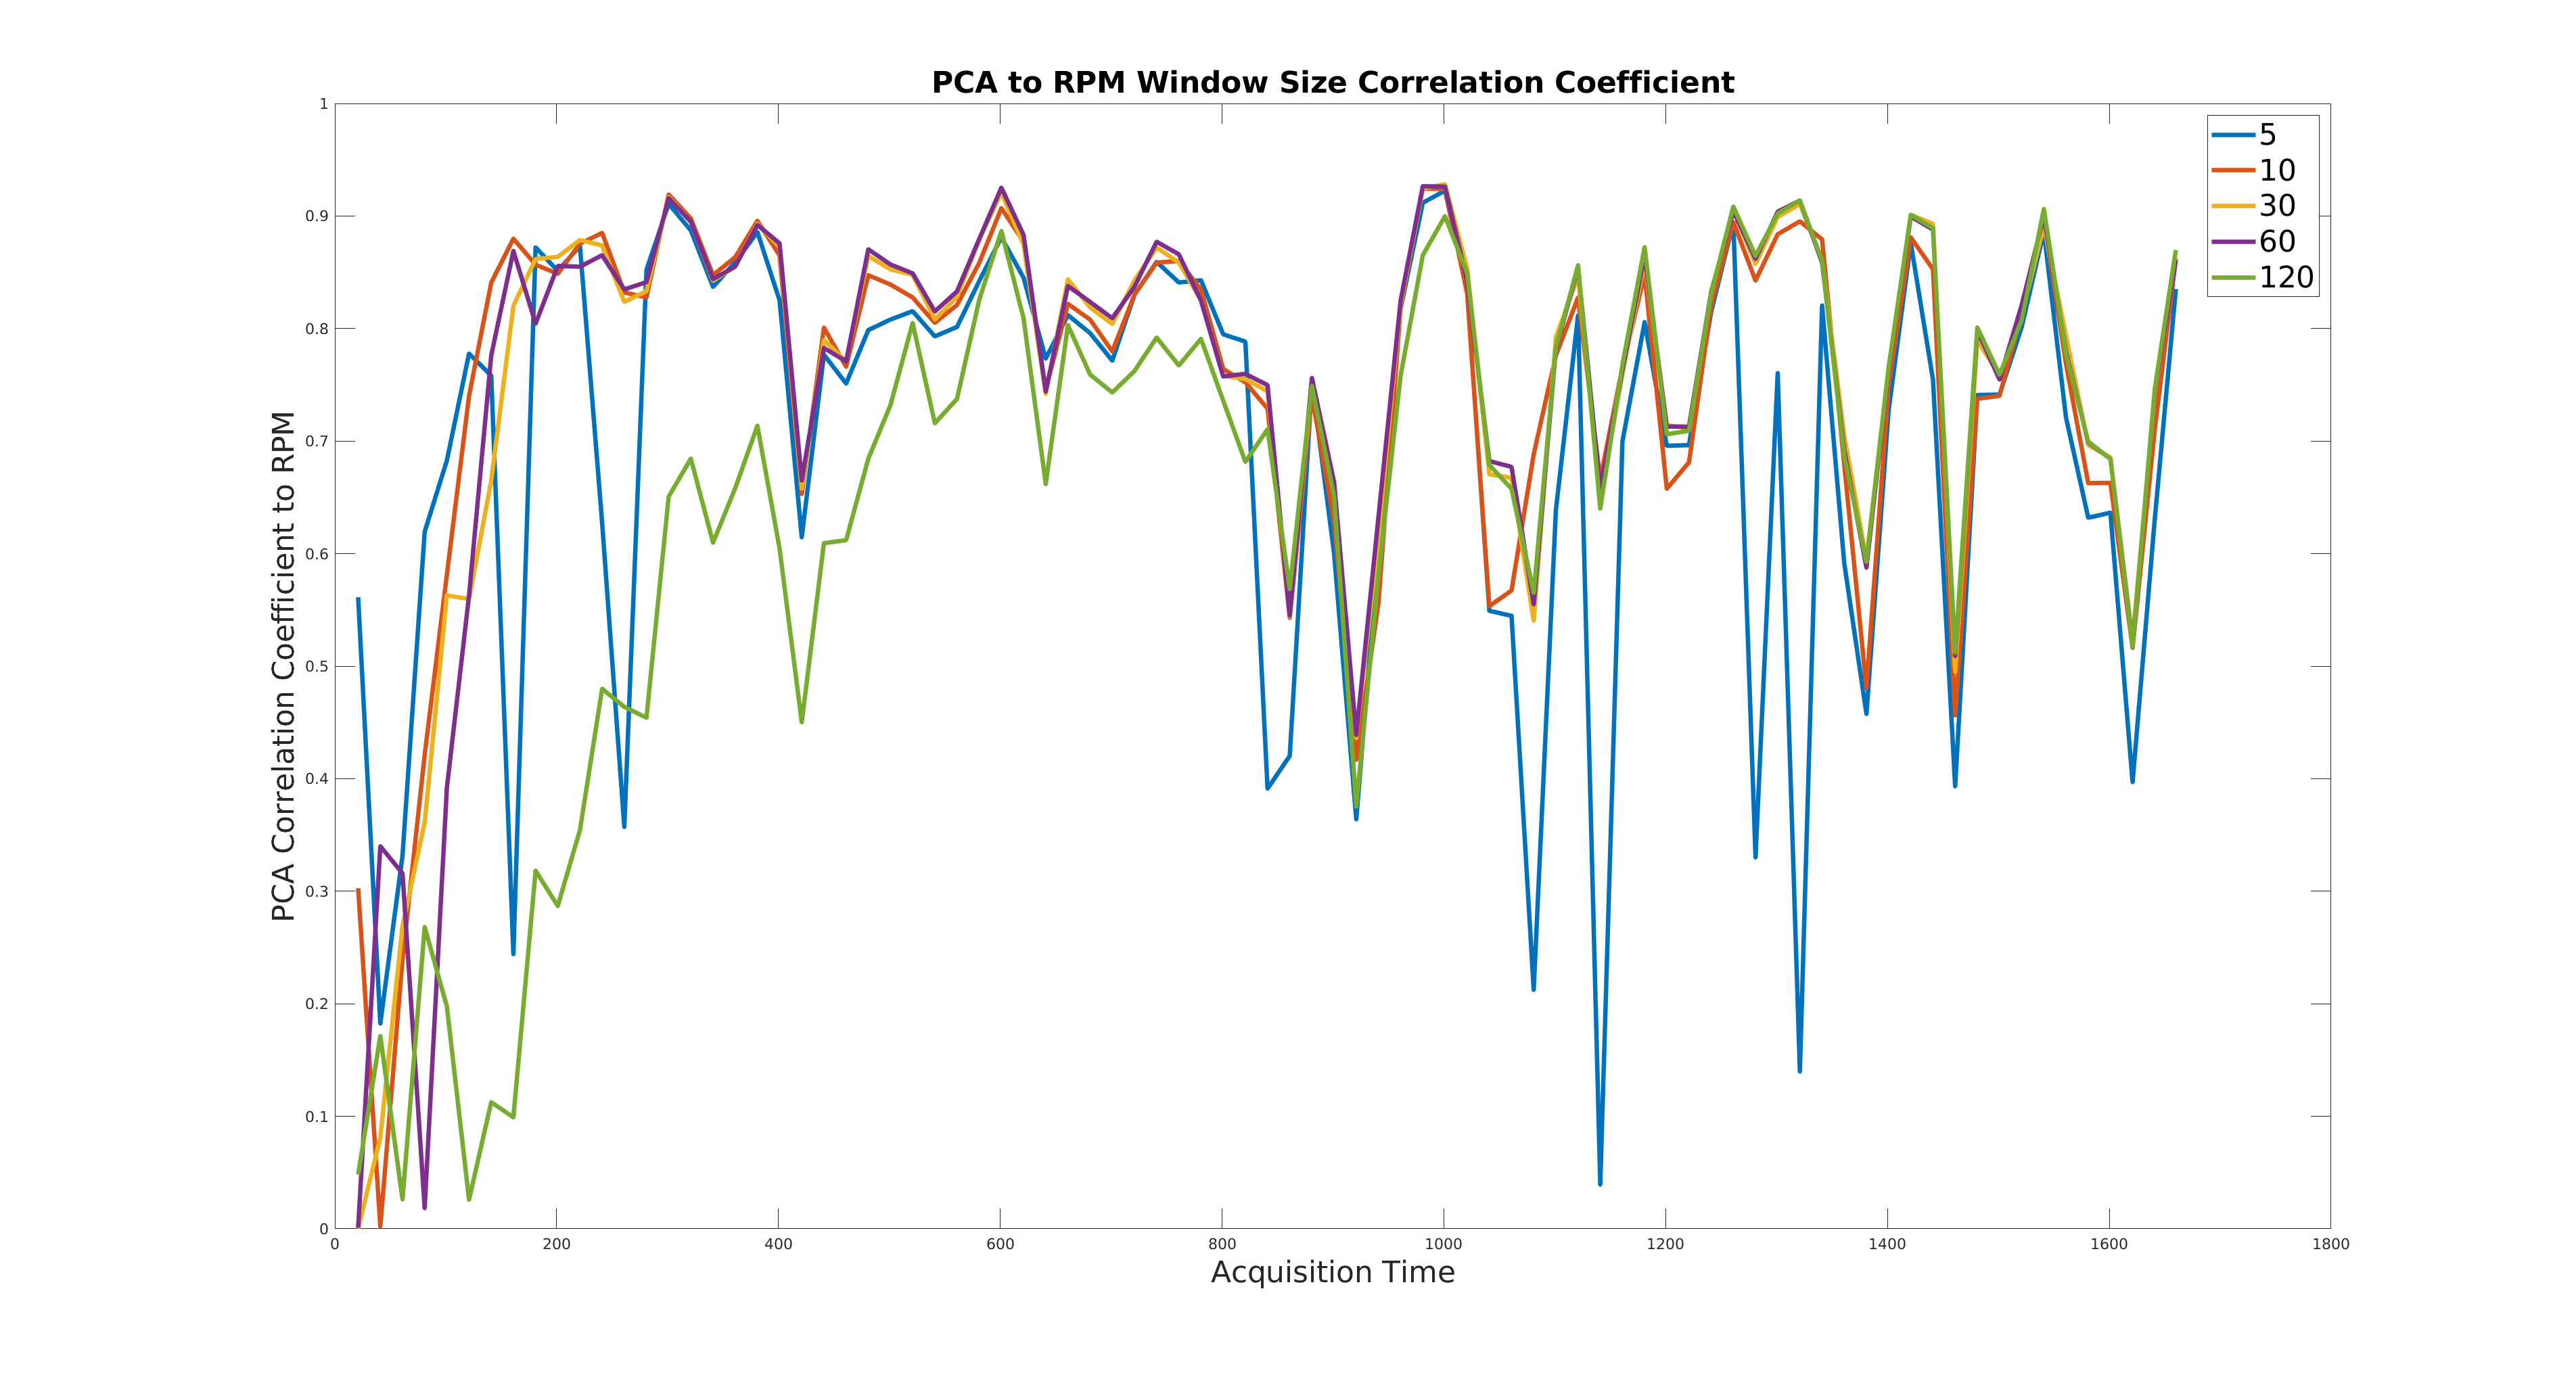
\includegraphics[width=1.0\linewidth]{figures/pca_window_correlation_coefficient.png}
            % 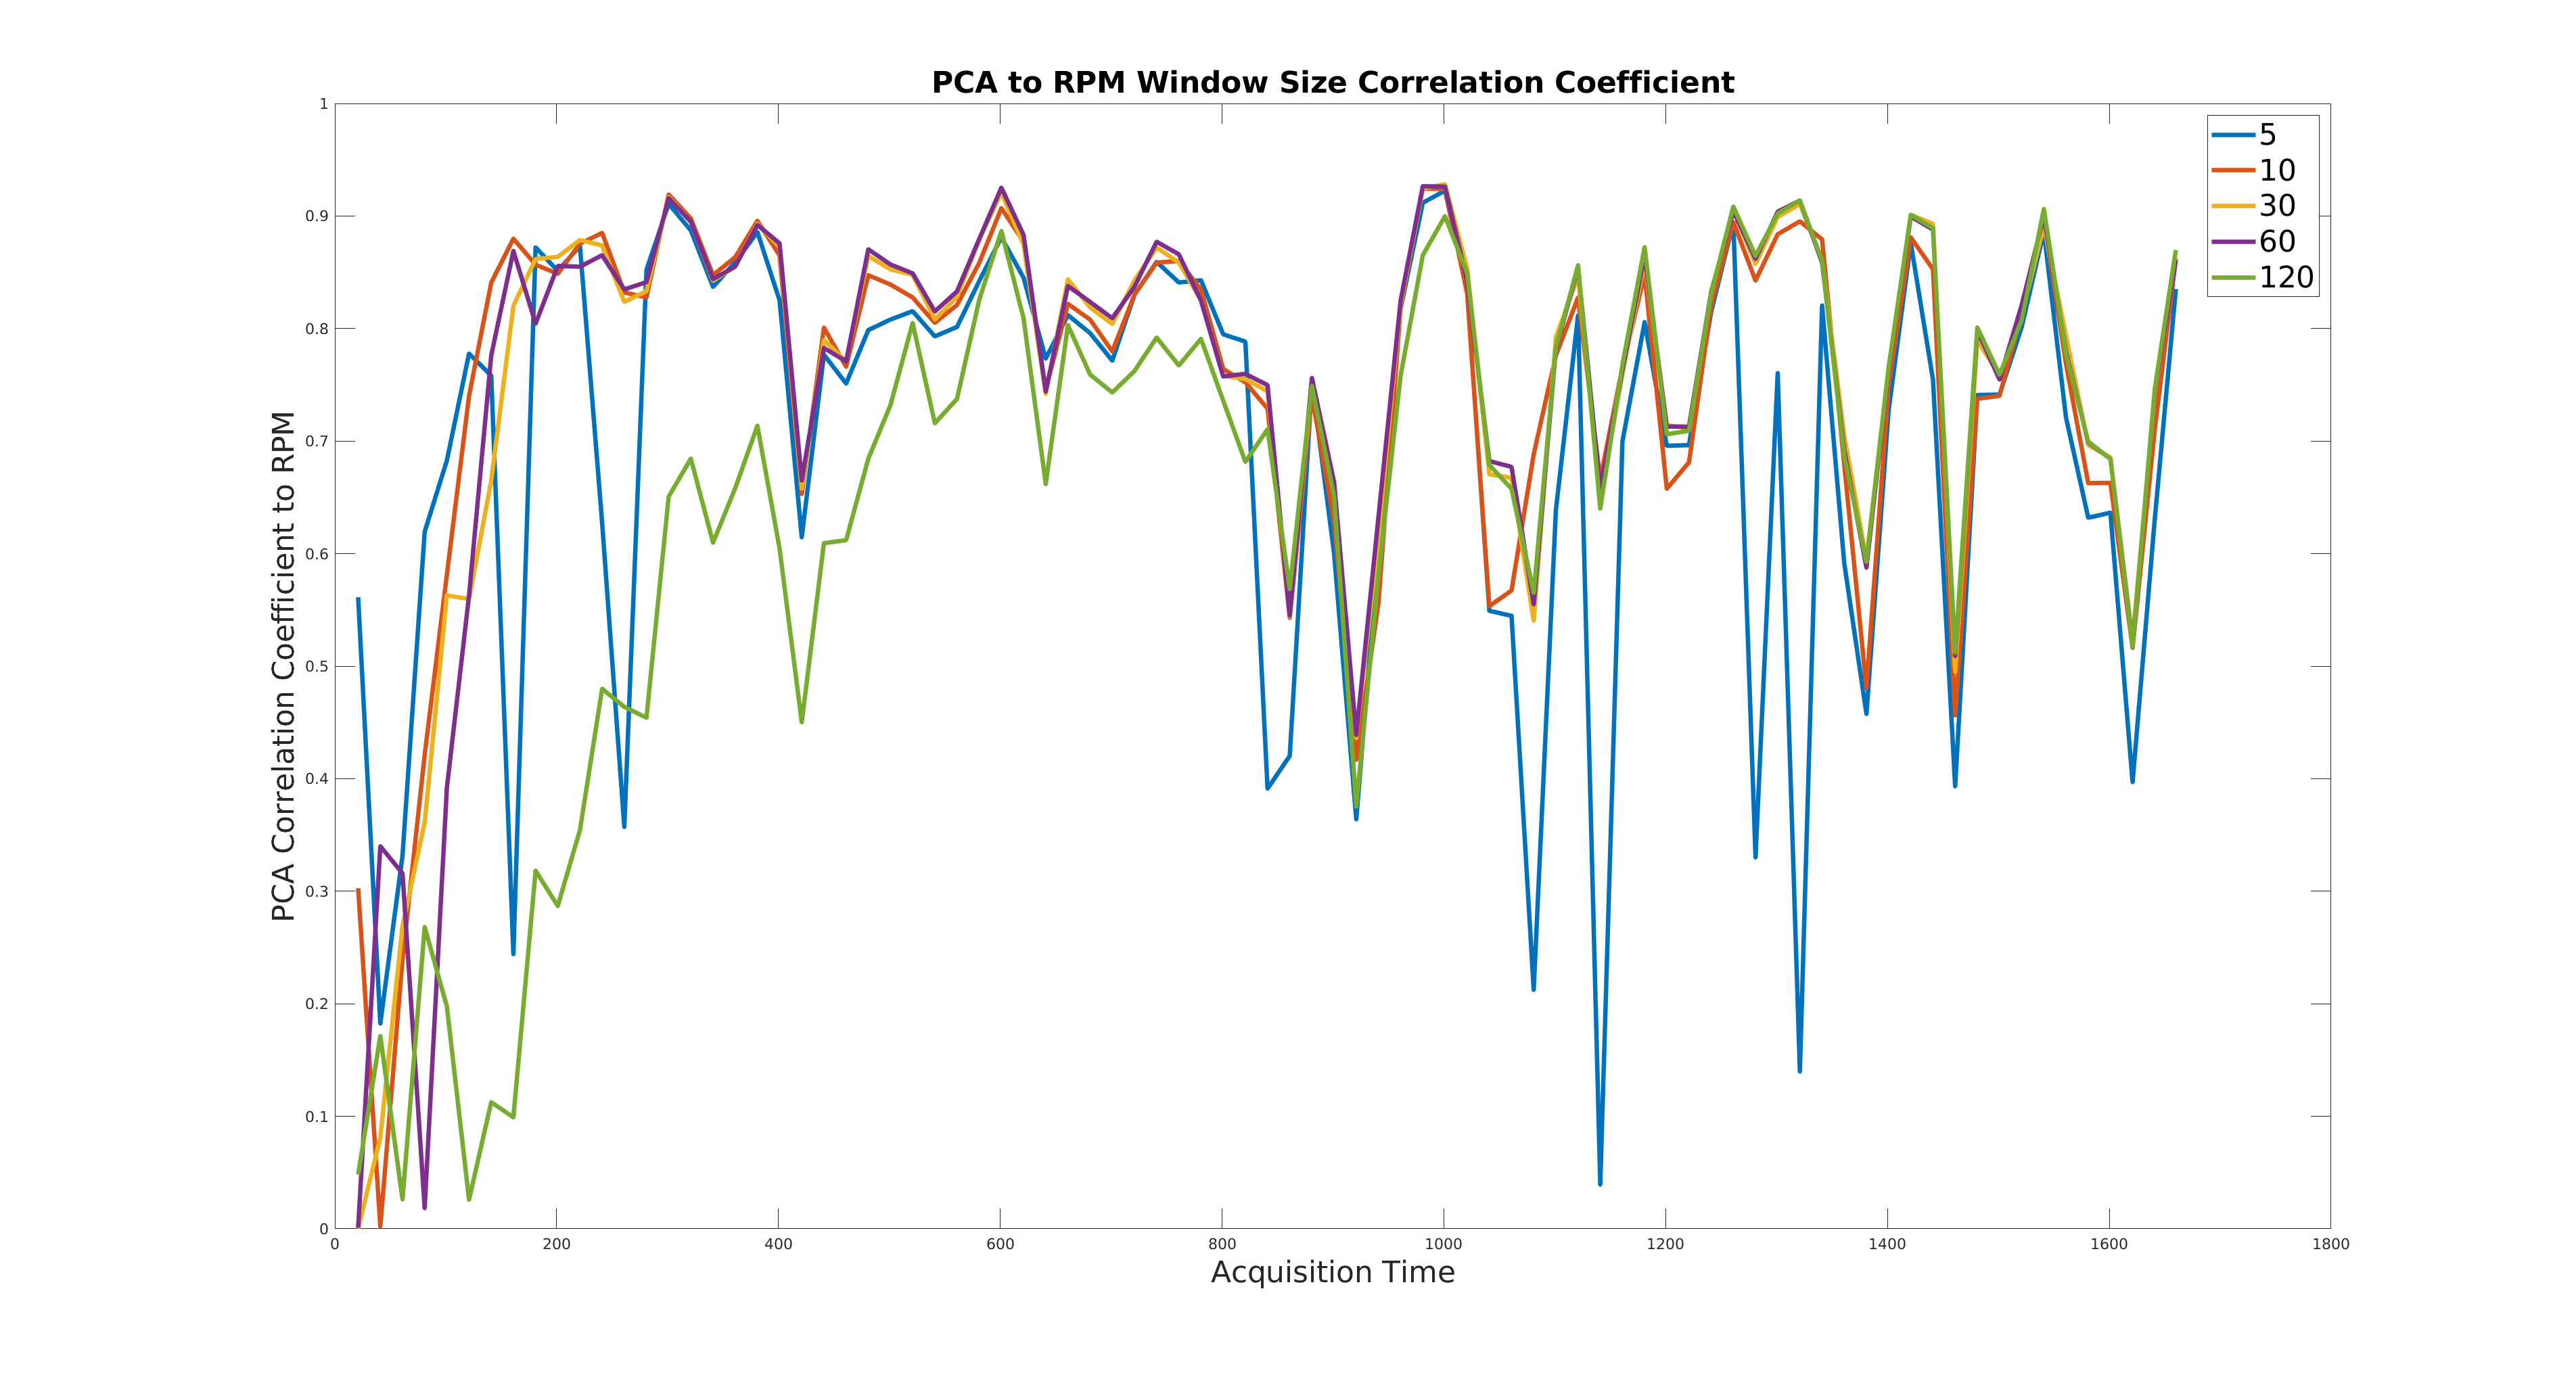
\includegraphics[width=1.0\linewidth]{figures/pca_window_correlation_coefficient.png}
            
            % \vspace{-0.4cm}
            
            \captionsetup{singlelinecheck=false, justification=centering}
            \caption{
            % \scriptsize
            A plot showing the Moving Window size optimisation for the \gls{PCA} method. For different fixed window sizes, the correlation of the extracted signal  to the \gls{RPM}  is shown for the windows sliding over the whole acquisition (taken for the first acquisition of patient one). Note that \SI{0.5}{s} time frames were used.}
            
            \label{fig:pca_window_correlation_coefficient}
            
            % \vspace{-0.5cm}
        \end{figure}
            
        % \begin{figure}
            % \vspace{-0.5cm}
            
        %     \centering
            
        %     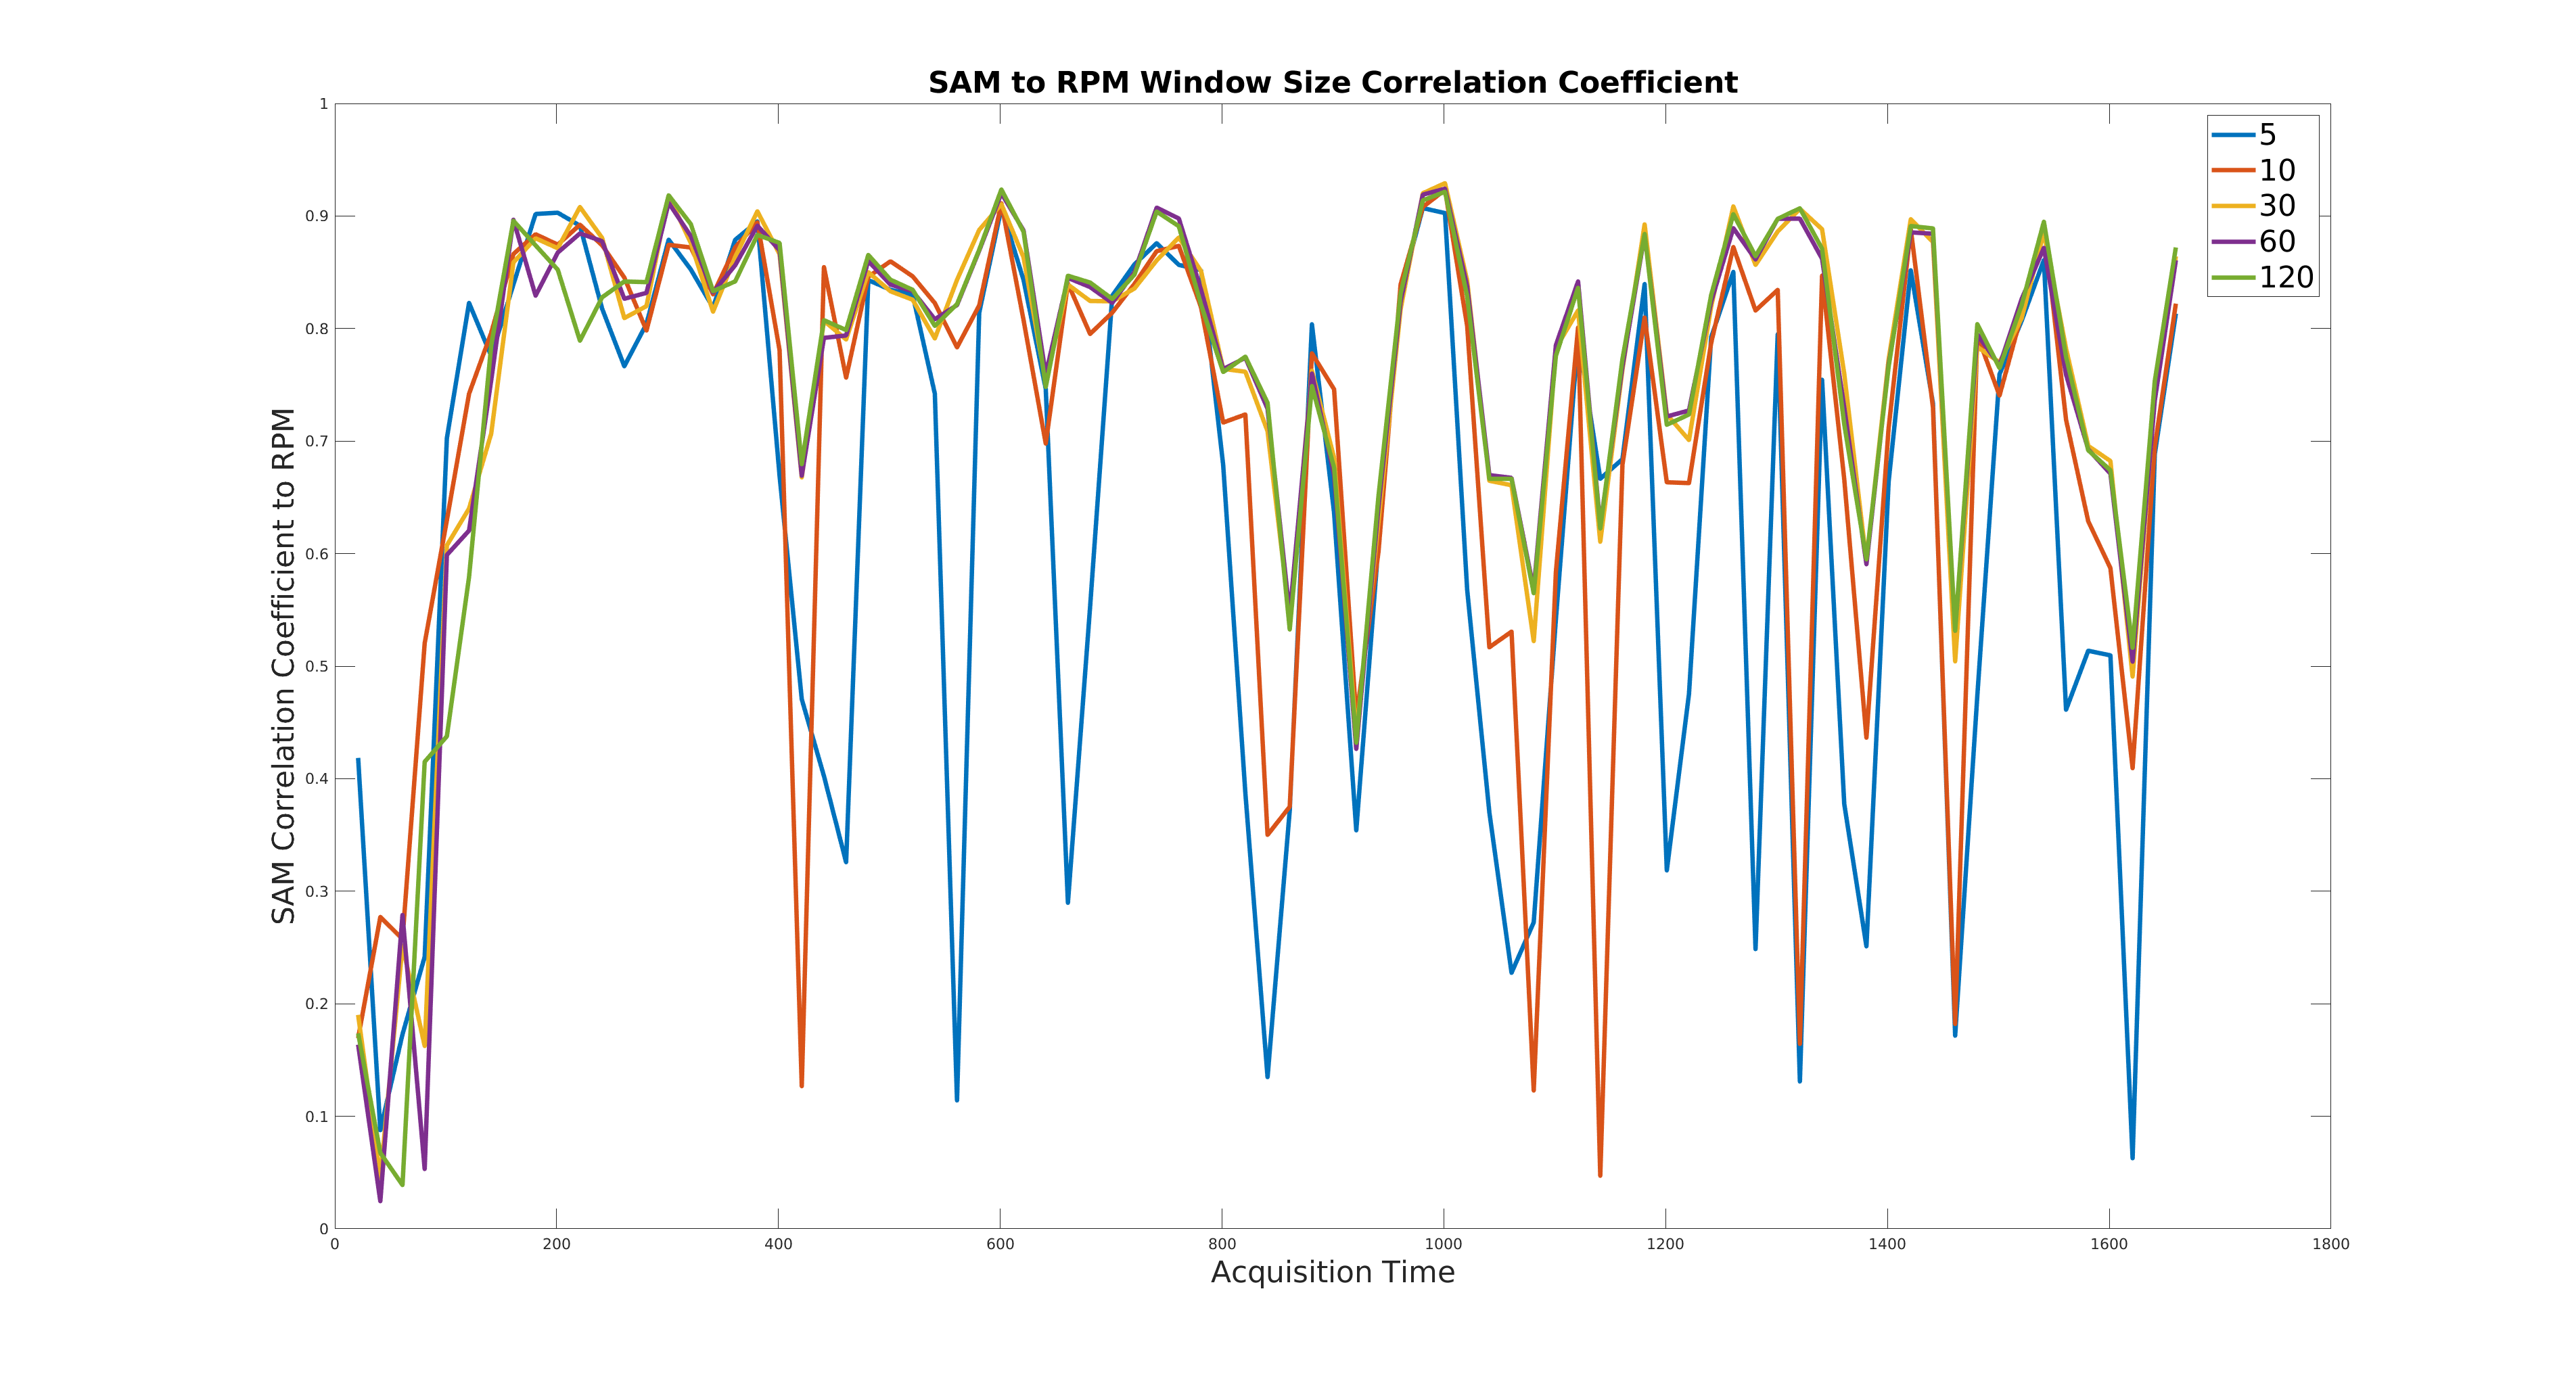
\includegraphics[width=1.0\linewidth]{figures/sam_window_correlation_coefficient.png}
            % 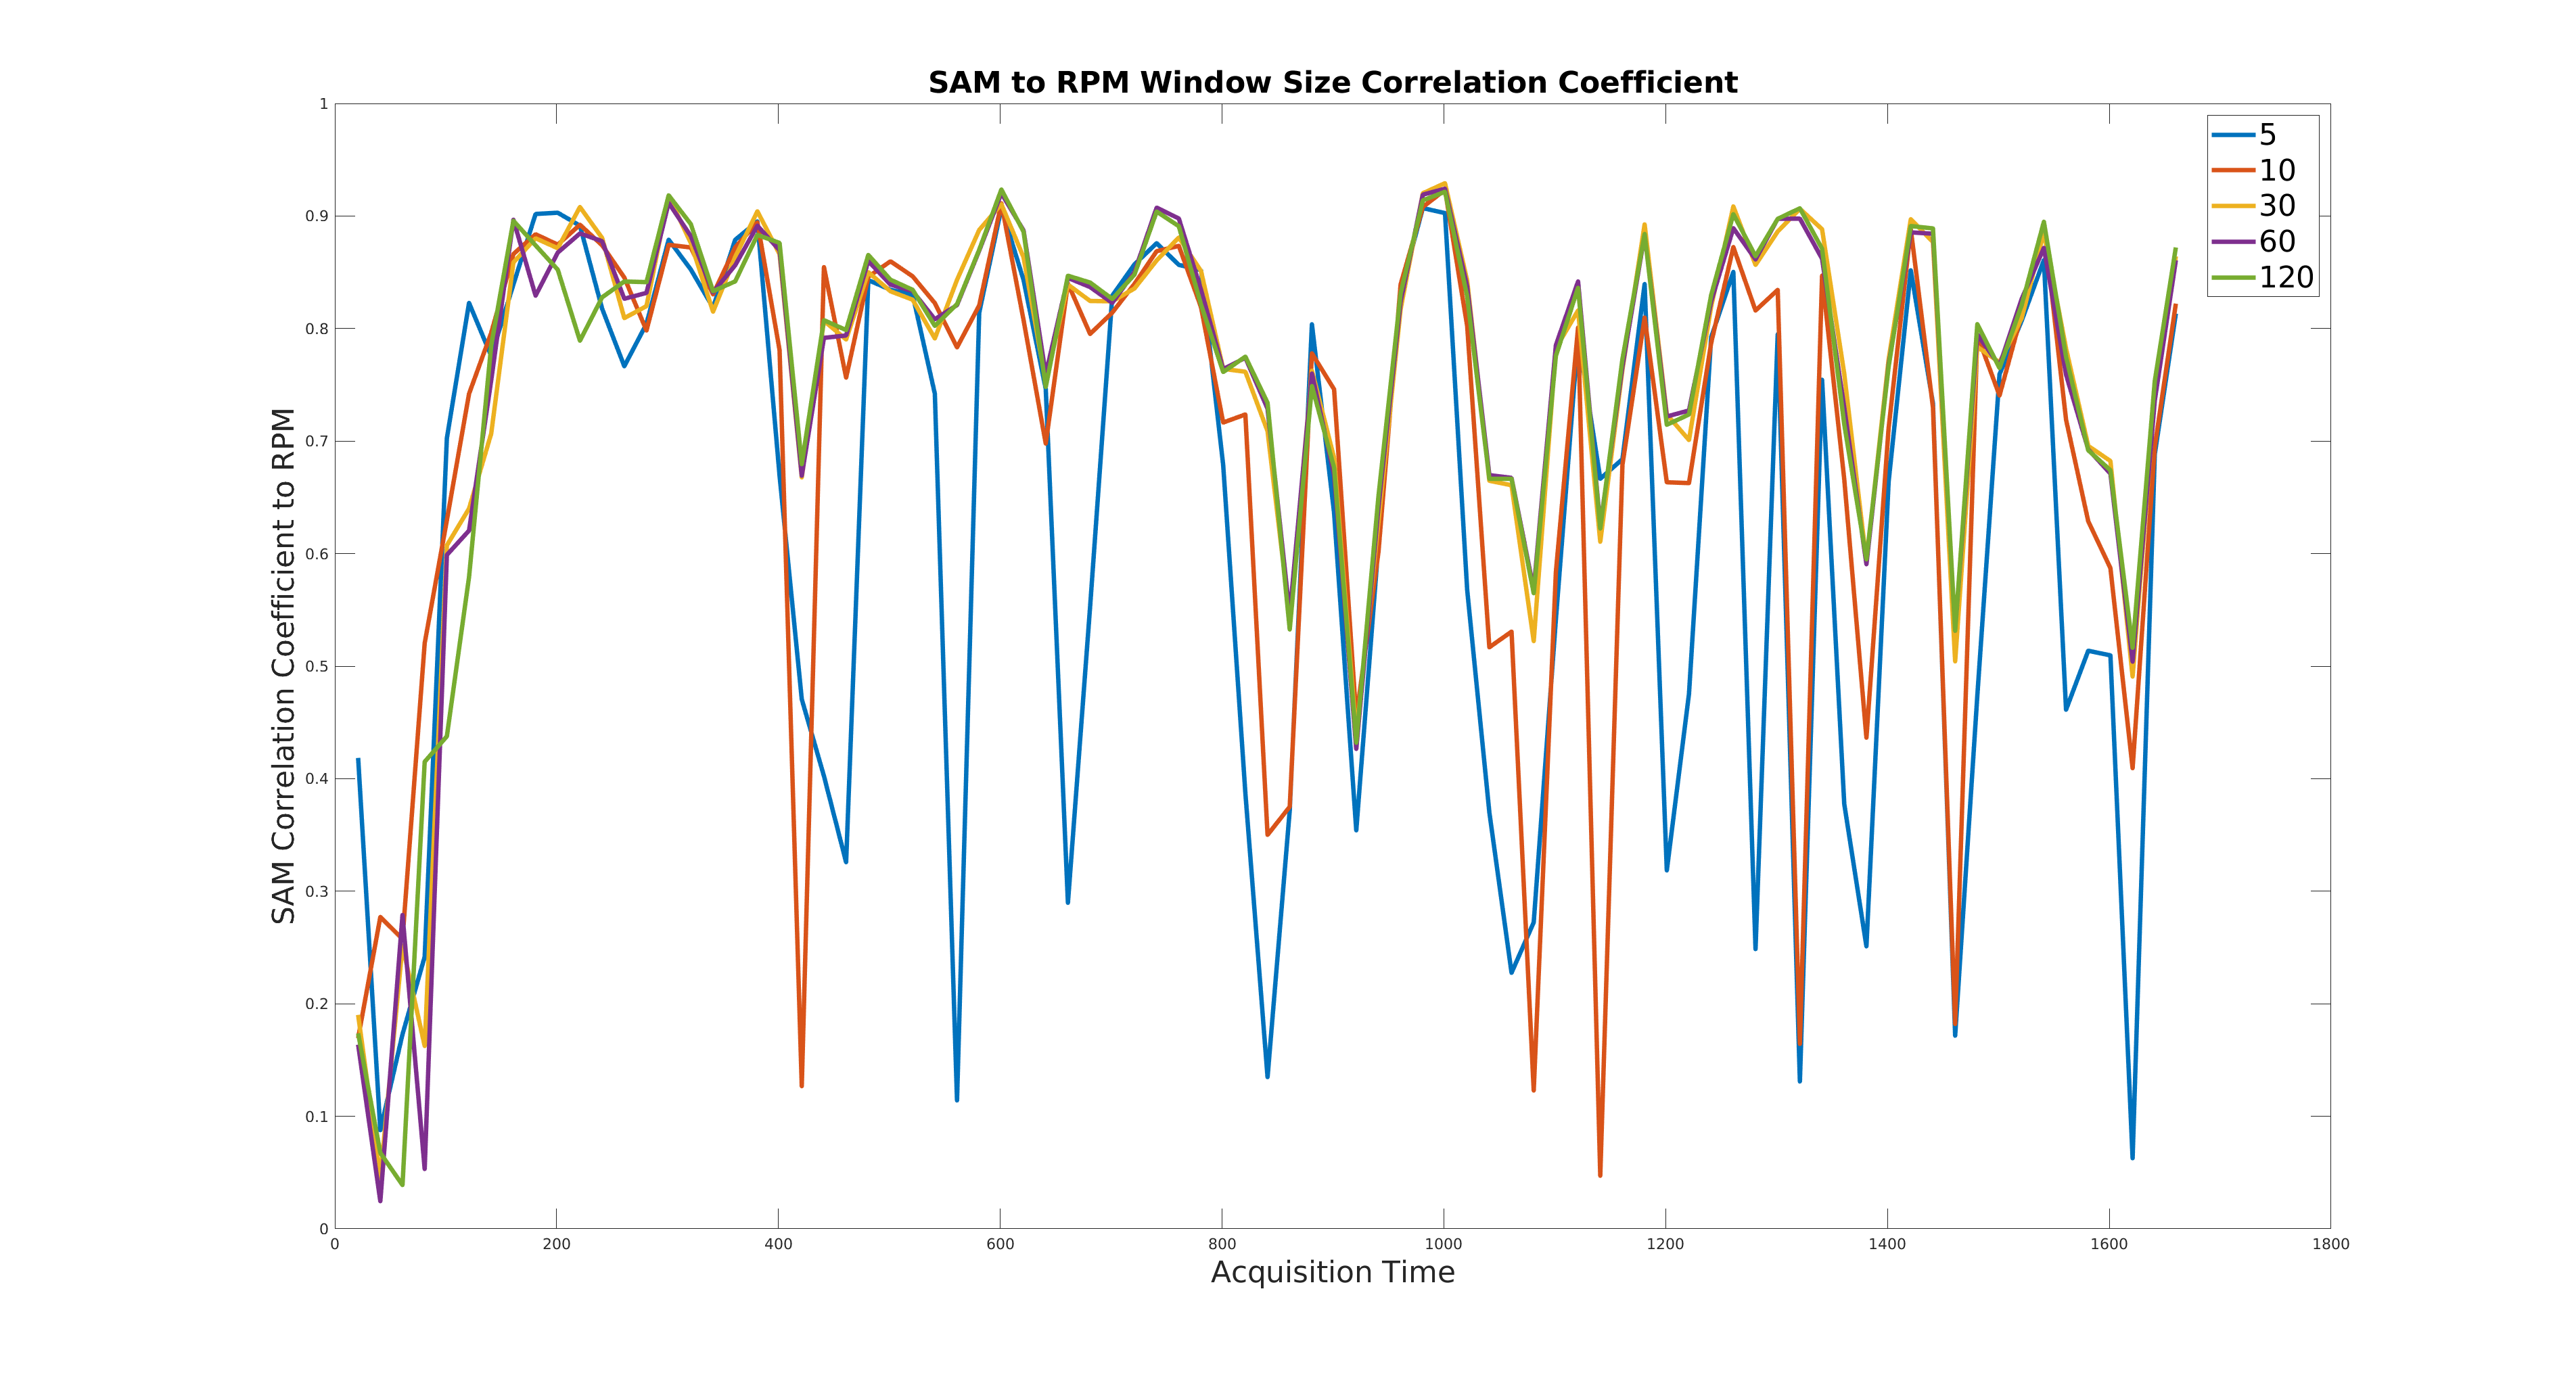
\includegraphics[width=1.0\linewidth]{figures/sam_window_correlation_coefficient.png}
            
            % \vspace{-0.4cm}
            
        %     \captionsetup{singlelinecheck=false, justification=centering}
        %     \caption{
            % \scriptsize
        %     A plot showing the Moving Window size optimisation for the \gls{SAM} method. For different fixed window sizes, the correlation of the extracted signal  to the \gls{RPM}  is shown for the windows sliding over the whole acquisition (taken for the first acquisition of patient one). Note that \SI{0.5}{s} time frames were used.}
            
        %     \label{fig:sam_window_correlation_coefficient}
            
            % \vspace{-0.5cm}
        % \end{figure}
    
        The data is split into a series of windows, where each subsequent window overlaps with the previous by half its length. The size of each window is predetermined and was selected experimentally. For this method \acrshort{PCA} is applied independently on each window, and the results are averaged together, after sign correction. As the sign of the signal from each window is arbitrary, the overlapping allows for a common sign to be found, by comparing the correlation coefficient of neighbouring windows. If \gls{SAM} is used here rather than \acrshort{PCA}, then the method approximates \gls{KRG}~\cite{Schleyer2014}.
        
        In~\Fref{fig:pca_window_correlation_coefficient}% and~\Fref{fig:sam_window_correlation_coefficient}
        , the Moving Window size optimisation for the \gls{PCA} %and \gls{SAM} 
        method can be seen.
        
    % \vspace{-0.5cm}
            
    \subsection{Late Time Point} \label{sec:late_time_point}
        A \gls{PC} from a late time point is taken, and used with early time point data. The cutoff between early and later time points was determined experimentally; by varying the cutoff point and observing the impact on the correlation coefficient, between the output and \gls{RPM} signal for the first \SI{120}{\second} (between \SI{20}{\second} and \SI{140}{\second}).
        
    % \vspace{-0.5cm}
    
    \subsection{Select and Combine} \label{sec:select_and_combine}
        Here a "respiratory score" is used to order and combine multiple \glss{PC} to maximise this score.
        
        \subsubsection{Selecting \glss{PC}} \label{sec:selecting_pcs}
              We used two methods for scoring:
              
              In the first, \gls{PSD} are calculated, and frequency windows representing the content of information related to radiotracer kinetics, respiratory motion, and noise are defined. The contribution within each window is determined for each \gls{PC}, by finding the maximum magnitude within the windows. Ratios are then calculated between the respiratory and the kinetic windows, and the respiratory and the noise windows and a score determined by the product of these two values.
        
        % % \vspace{-0.5cm}
        
        %\subsubsection{Selecting \glss{PC} Using A Neural Network} \label{sec:selecting_pcs_using_a_neural_network}
            In the second, a \gls{NN} was used for scoring. The \gls{NN} is a pre-trained model, designed to accept a signal as input, and return a score between $0.0$ and $1.0$, where the greater the value the more respiratory-like the signal. The \gls{NN} was originally trained on a similar set of training data, where the scores were predetermined by clinicians~\cite{Walker2020AutomaticAI}.
        
        % % \vspace{-0.5cm}
        
        \subsubsection{Combining \glss{PC}} \label{sec:combining_pcs}
            \glss{PC} are first sorted according to the score. The sorted \glss{PC} are iterated over and both summed and subtracted with a weighting (the score), and a new score is found for both resulting signals. If one of the signals increases the score, it becomes the new best \gls{PC}, and goes forward to the next iteration. \glss{PC} are both summed and subtracted to handle the arbitrary sign problem.
            
            A similar method of combining signals was developed in~\cite{Kesner2010AMethods}. However, the scoring method used there (standard deviation) is not directly related to respiration. In addition,~\cite{Kesner2010AMethods} combined signals from voxels where our methods uses \glss{PC}.
        
    % \vspace{-0.5cm}
            
    \subsection{Evaluation} \label{sec:evaluation}
        For evaluation of the results, the correlation coefficient of each \gls{SS} between each method and the \gls{RPM}, for all acquisitions, has been calculated. The correlation coefficient has been calculated for both the first \SI{120}{\second}, and also the entire acquisition.
    
% \vspace{-0.4cm}
            
\section{RESULTS} \label{sec:results}
    \begin{figure}
        % \vspace{-0.5cm}
        
        \centering
        
        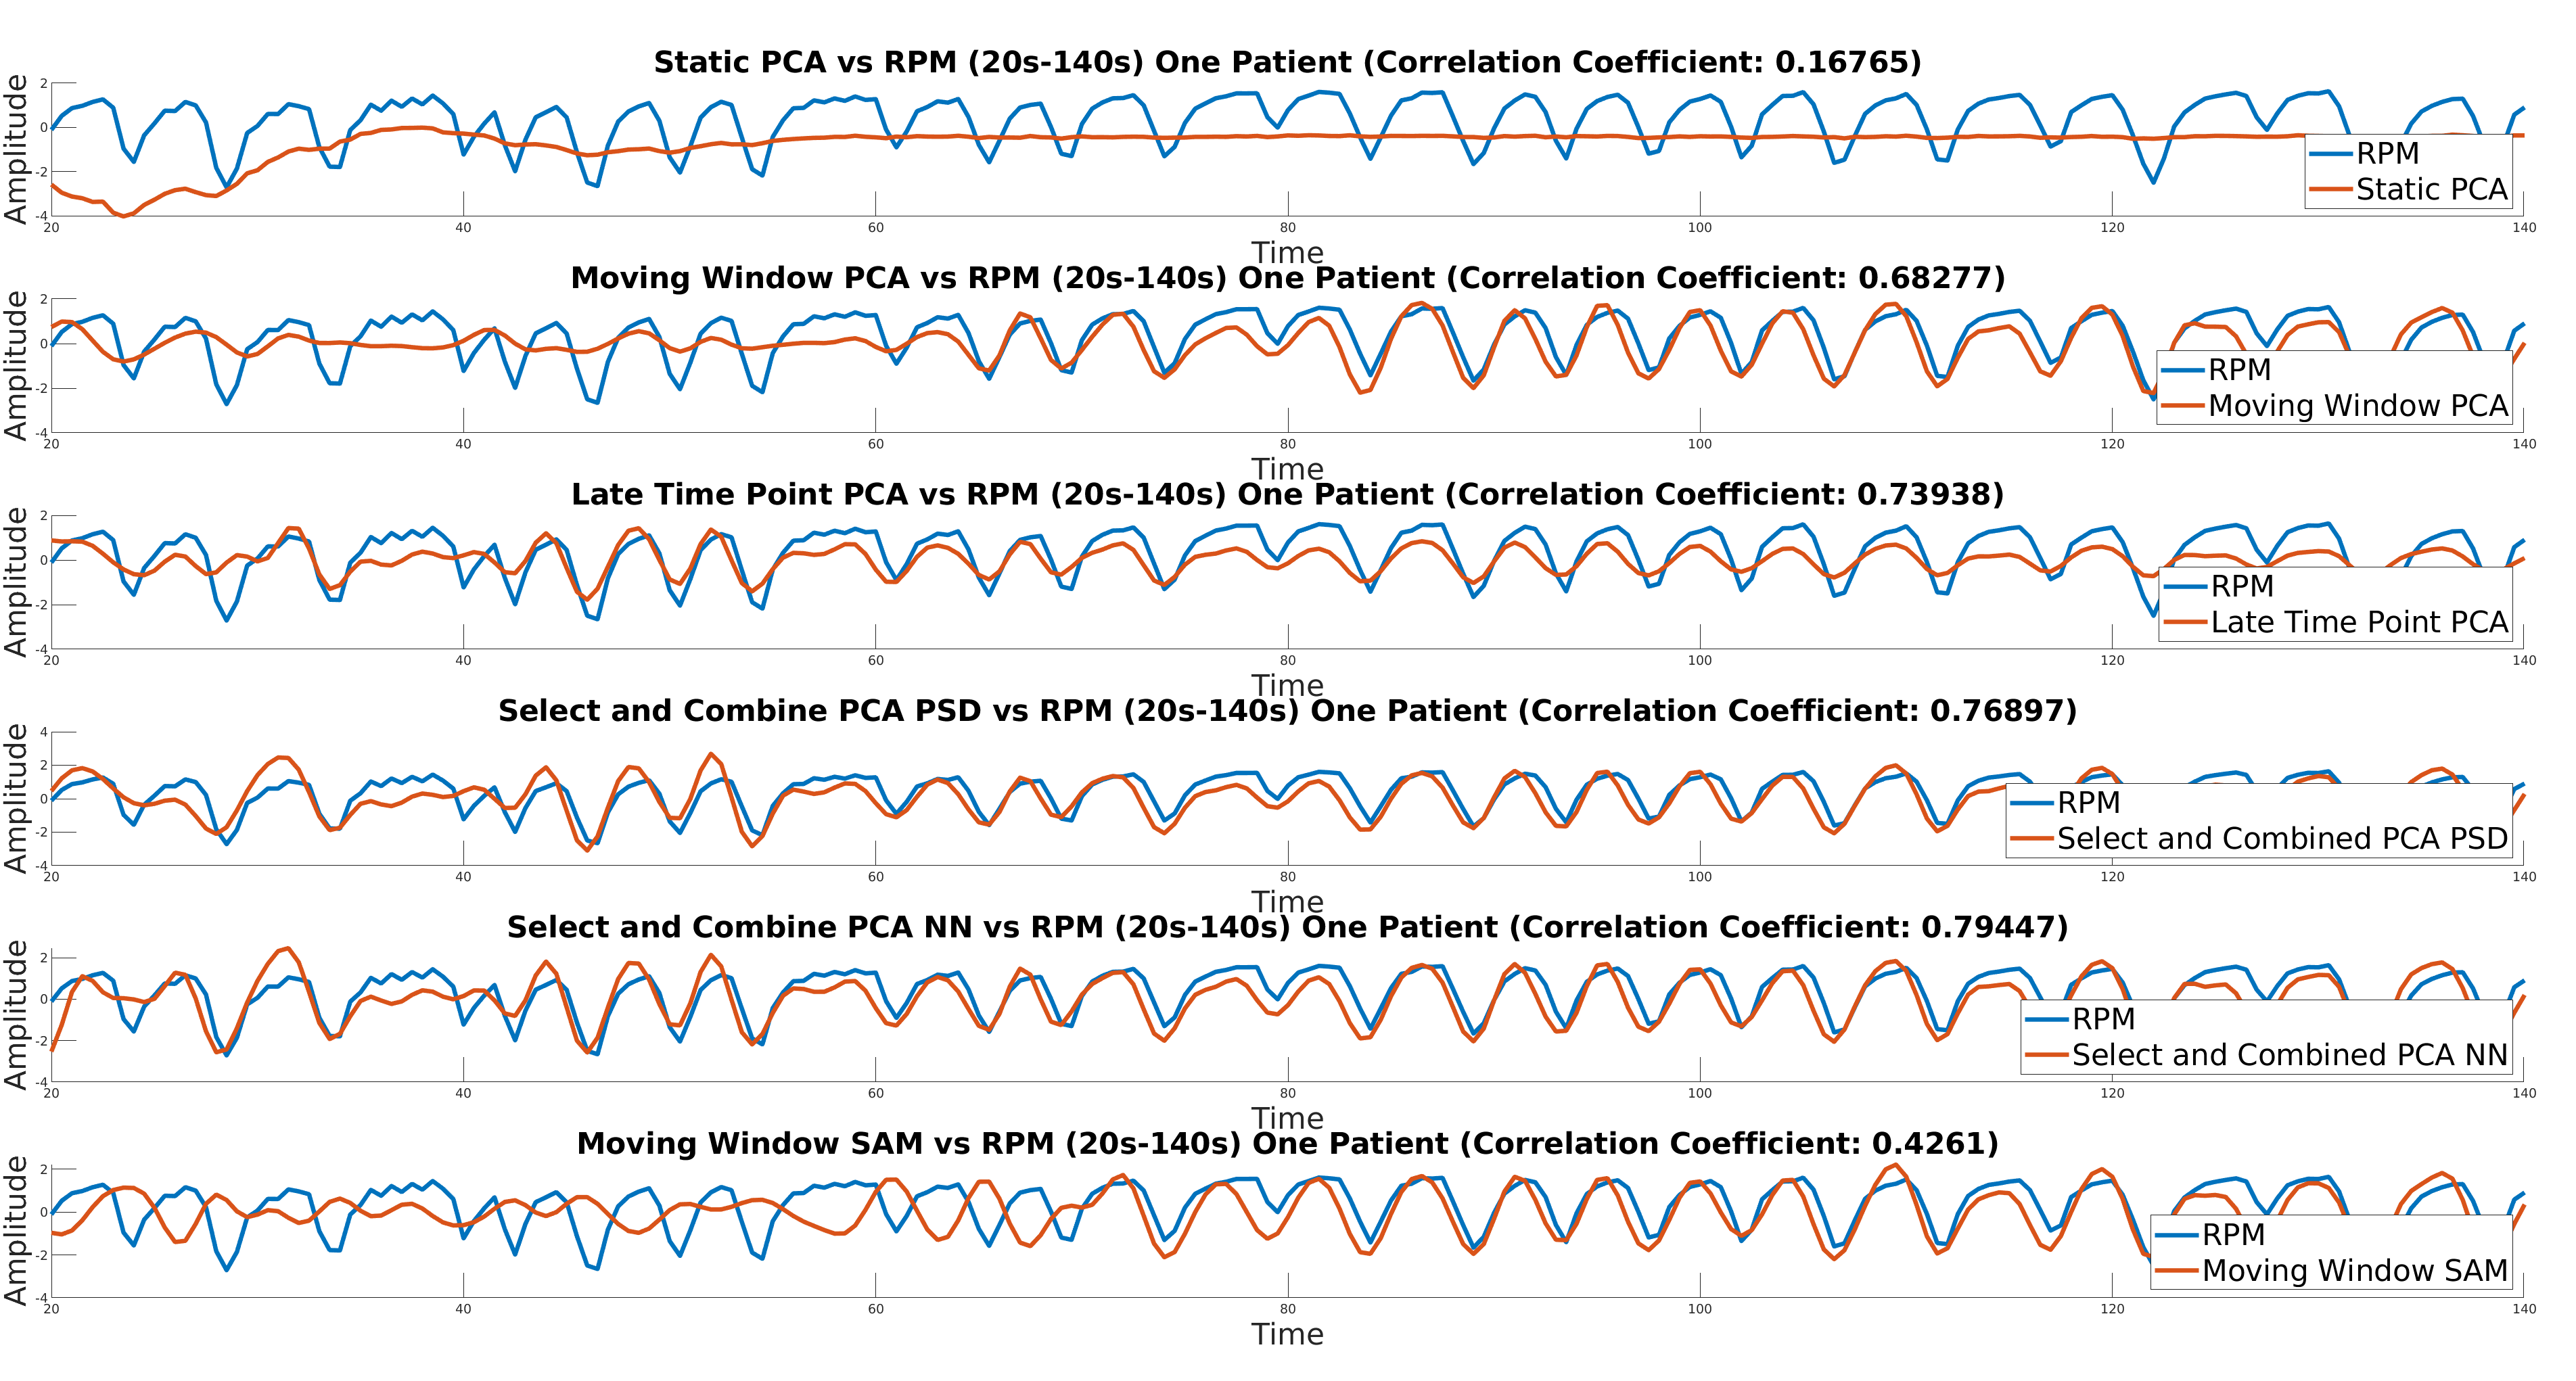
\includegraphics[width=1.0\linewidth]{figures/patient_one_output.png}
        % 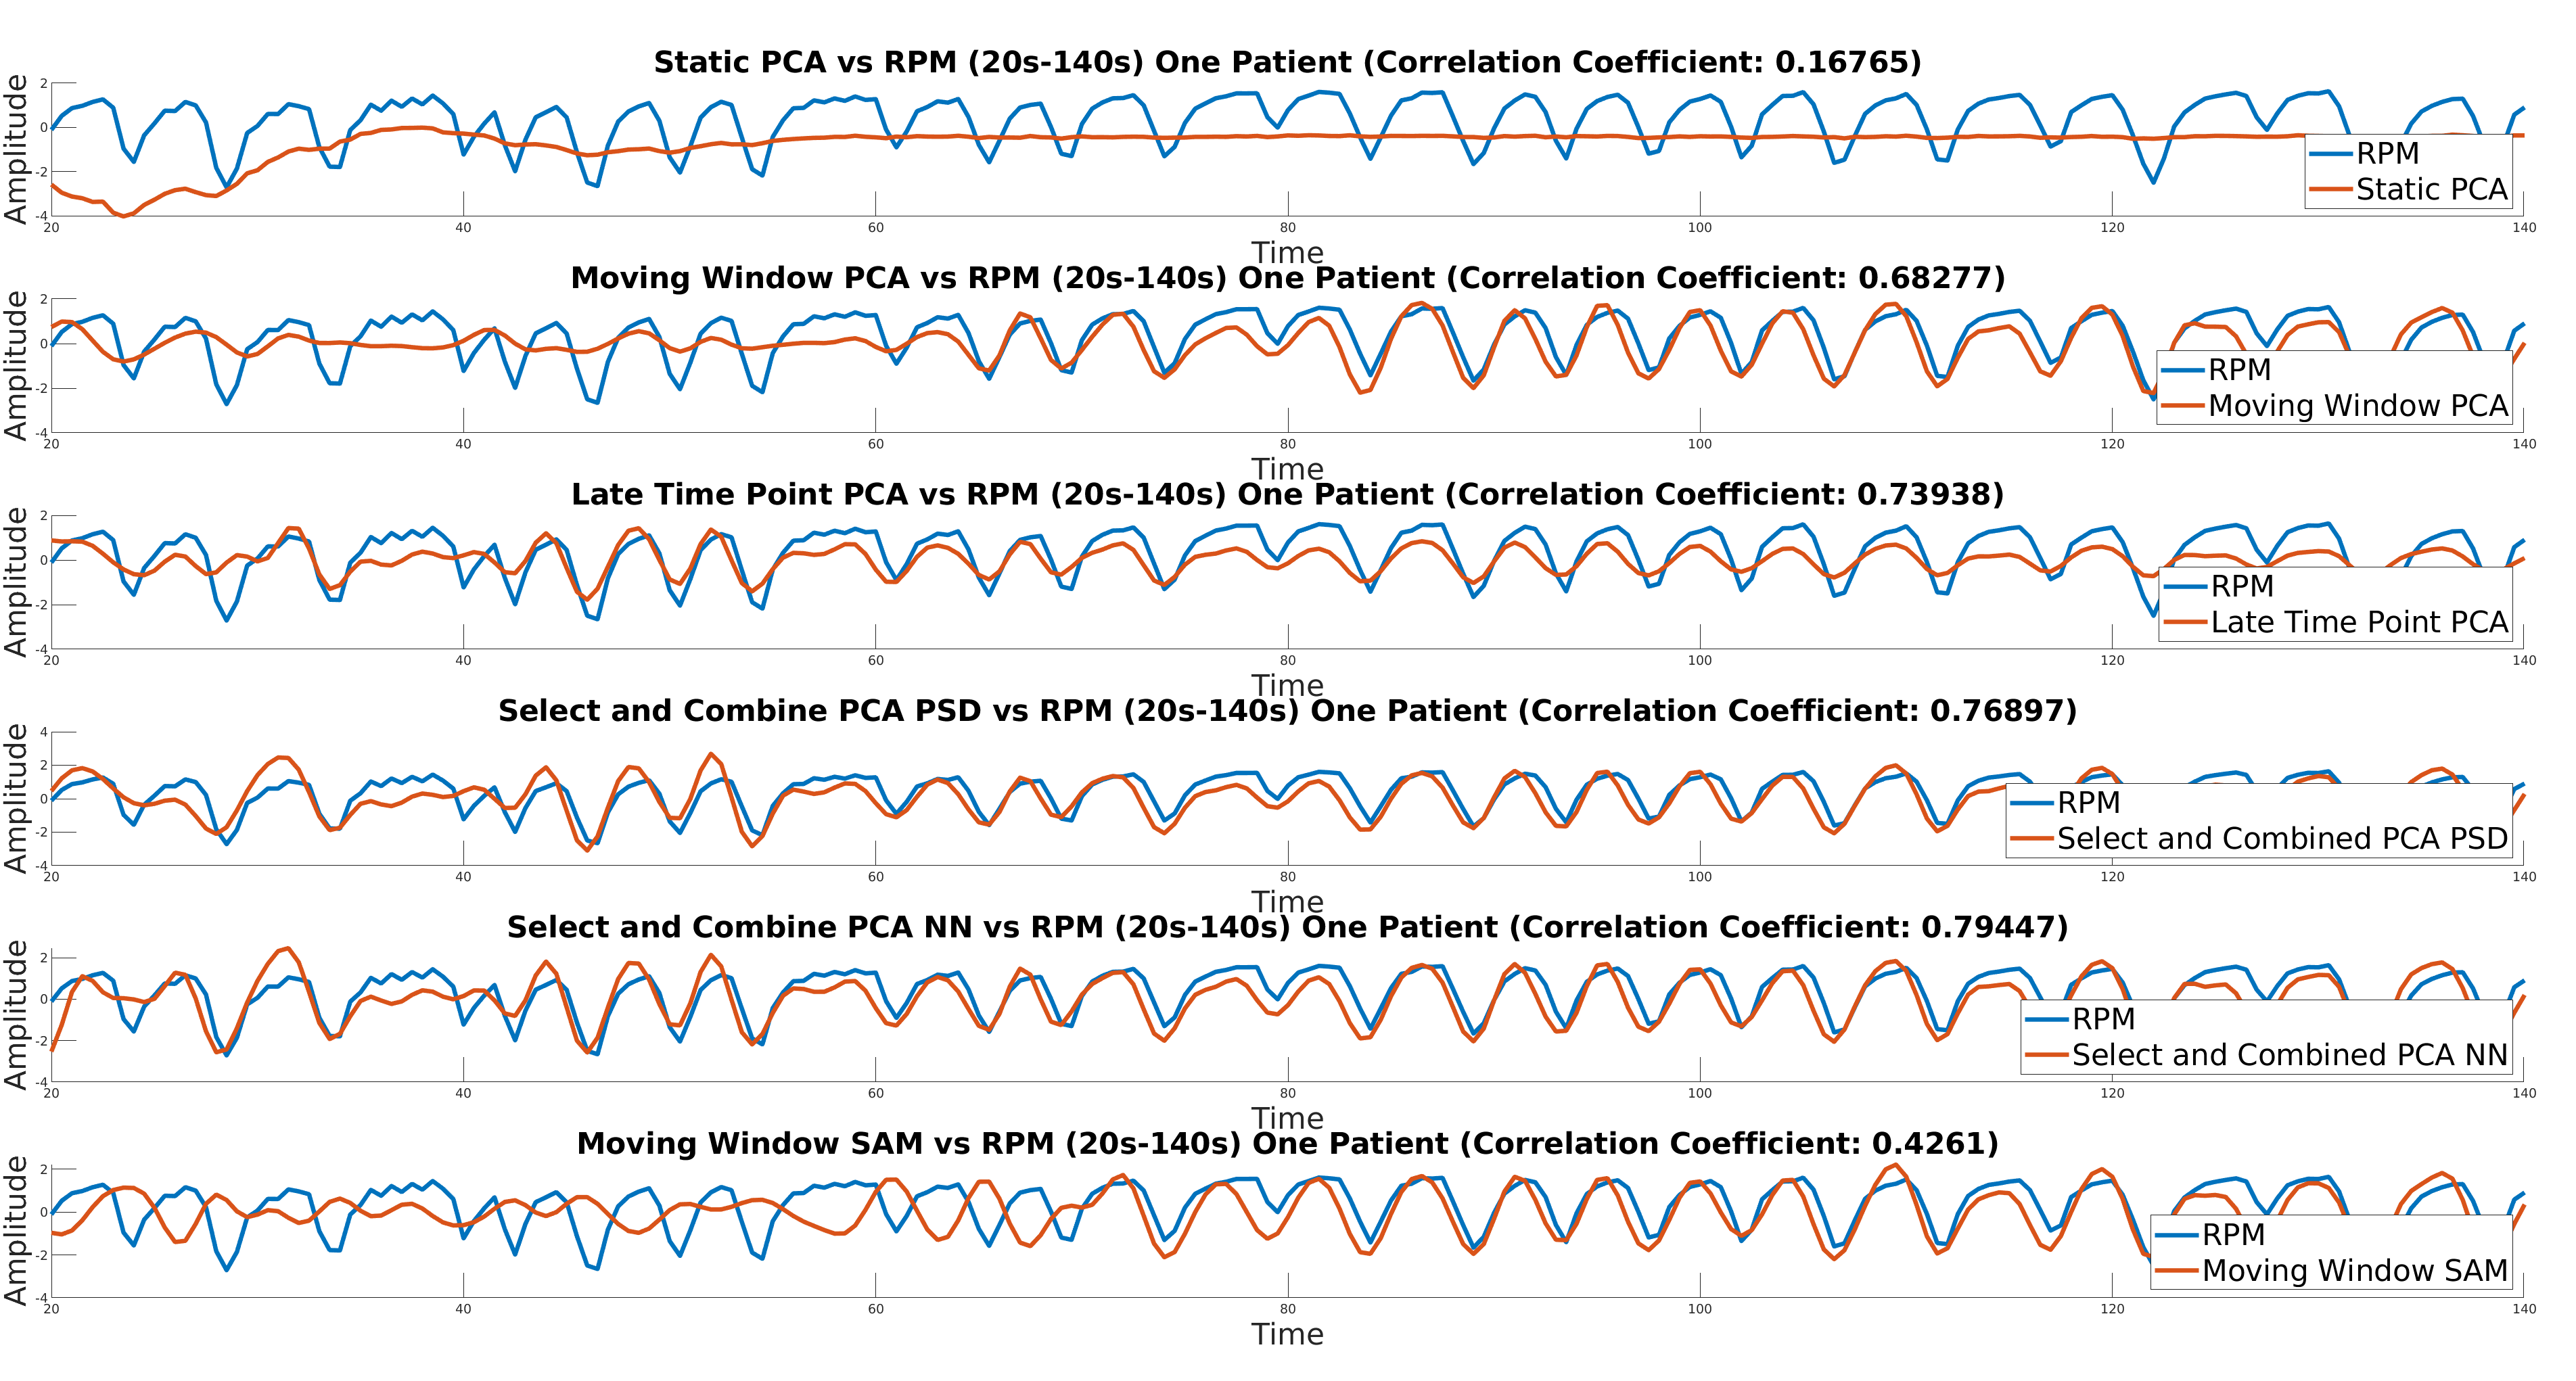
\includegraphics[width=1.0\linewidth]{figures/patient_one_output.png}
        
        % \vspace{-0.4cm}
        
        \captionsetup{singlelinecheck=false, justification=centering}
        \caption{
        % \scriptsize
        A plot showing for each method its output compared to the \gls{RPM} for the first \SI{120}{\second} (between \SI{20}{\second} and \SI{140}{\second}) (taken for the first acquisition of patient one).}
        
        \label{fig:patient_one_output}
        
        % \vspace{-0.5cm}
    \end{figure}
    
    \begin{figure}
        % \vspace{-0.5cm}
        
        \centering
        
        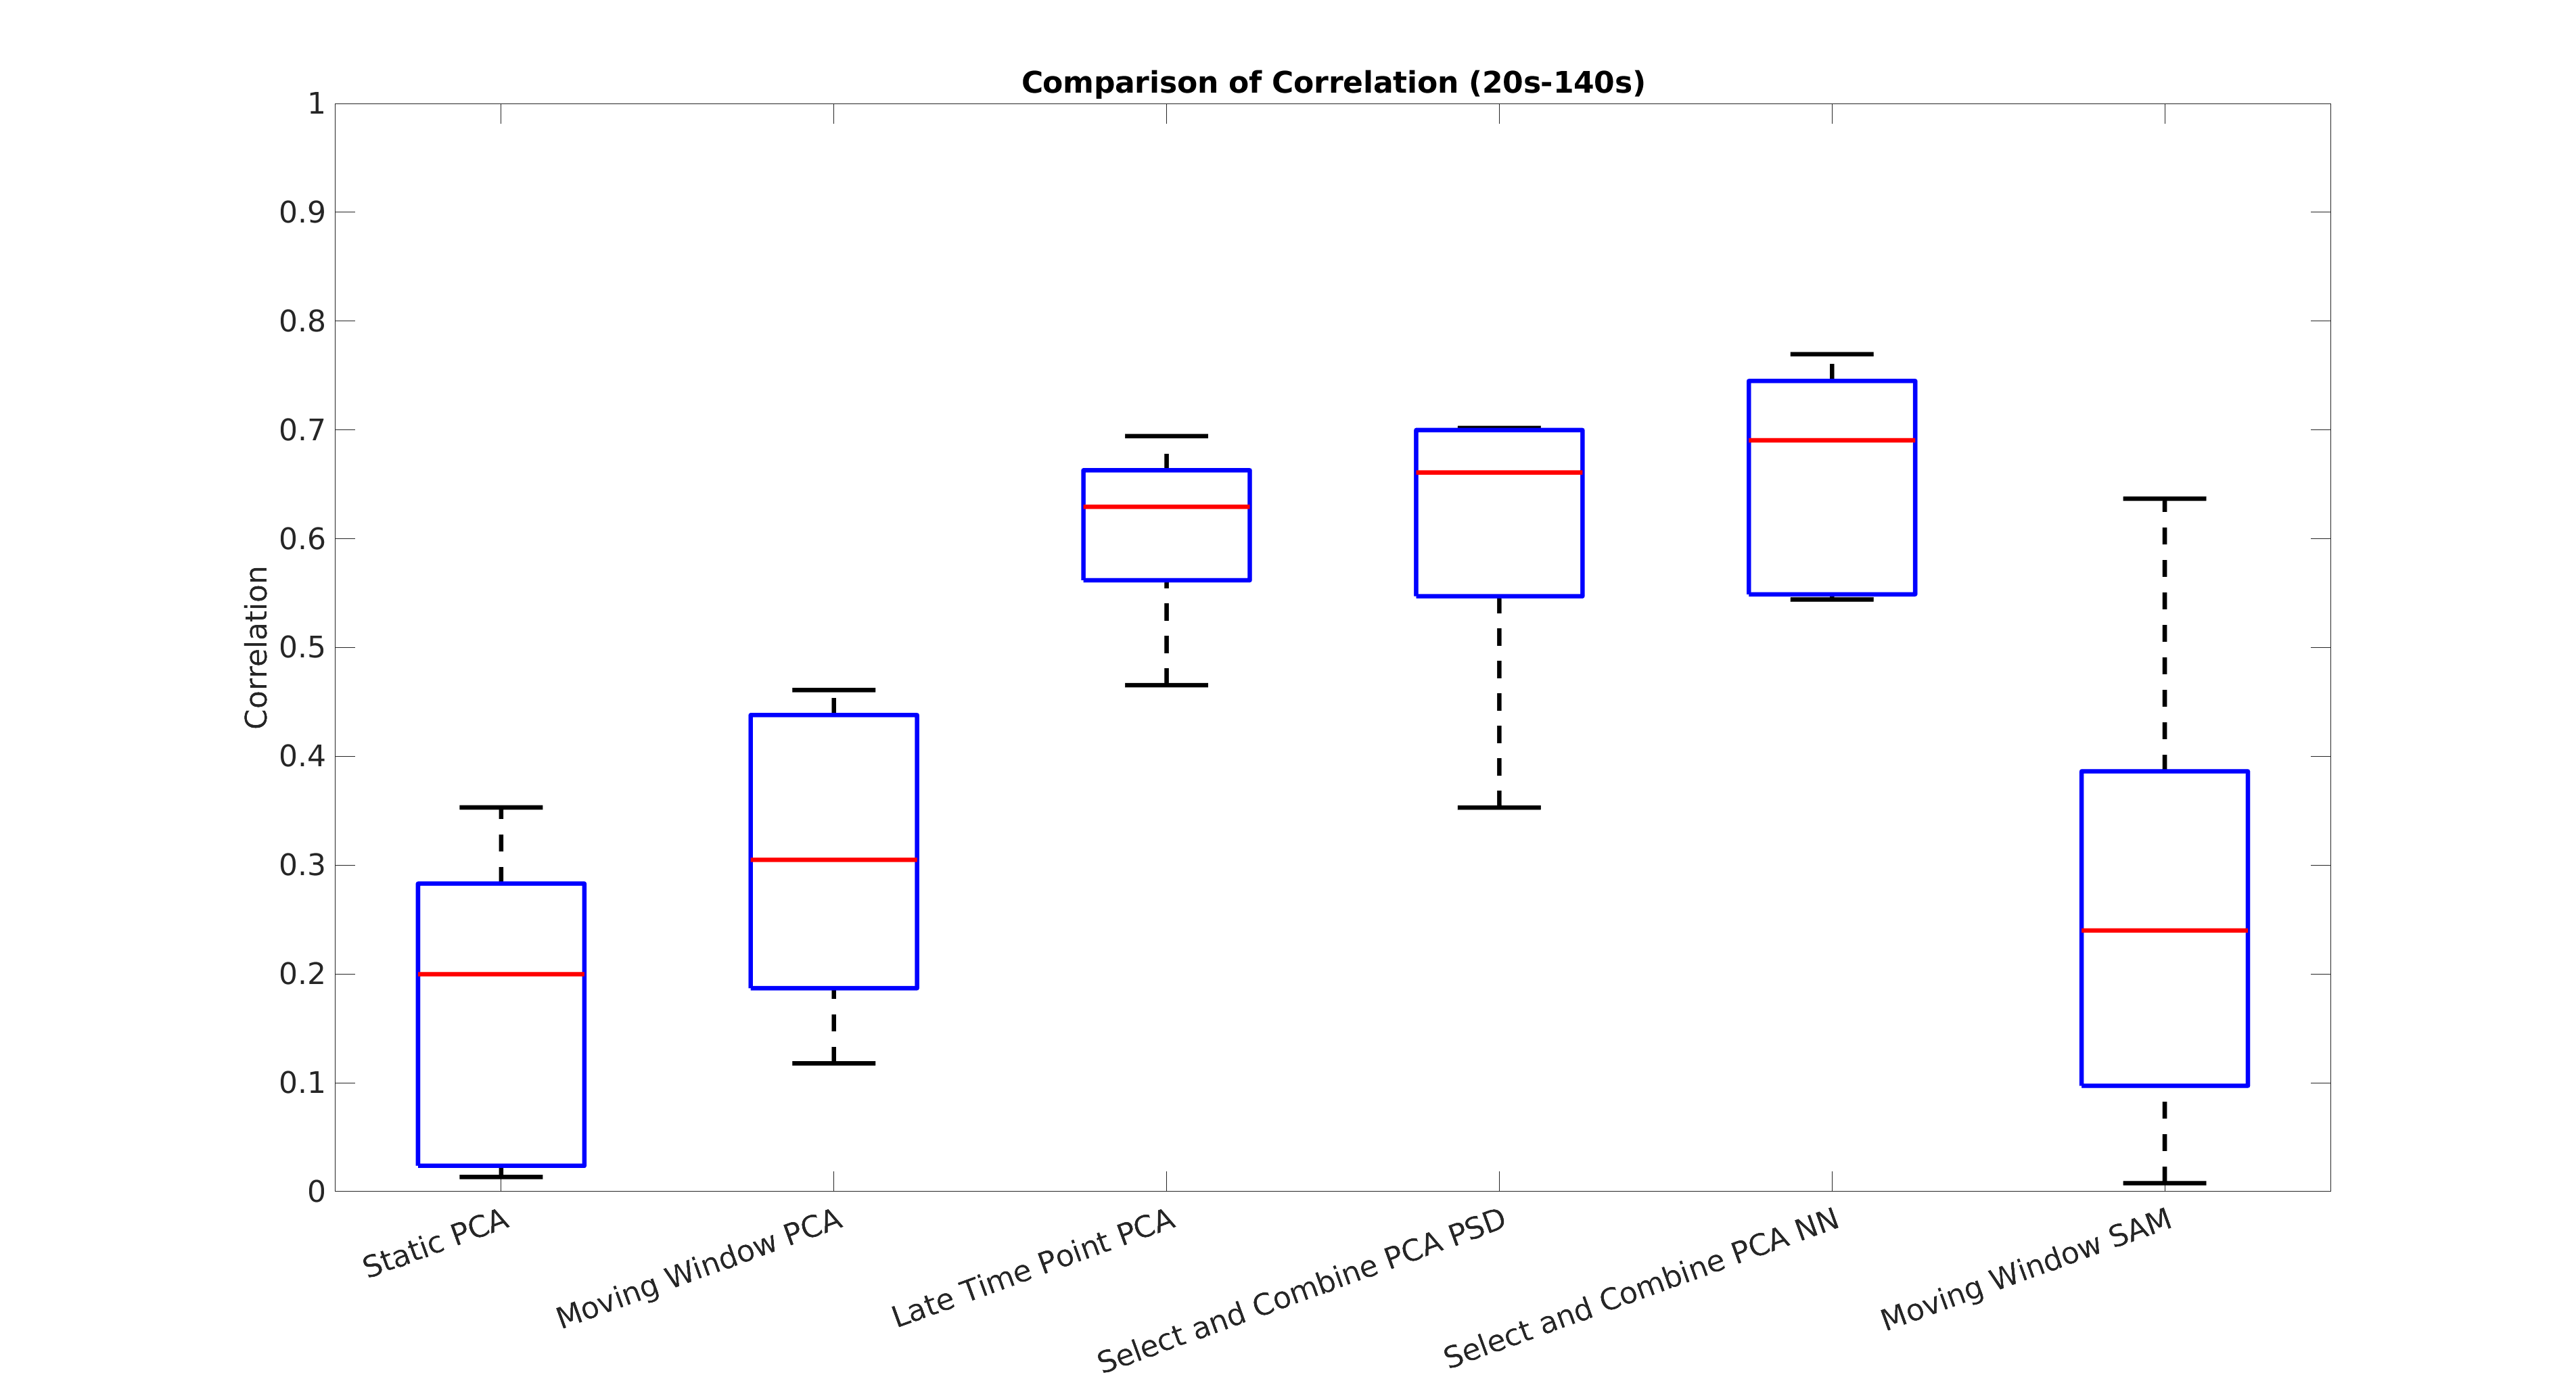
\includegraphics[width=1.0\linewidth]{figures/box_plot_early.png}
        % 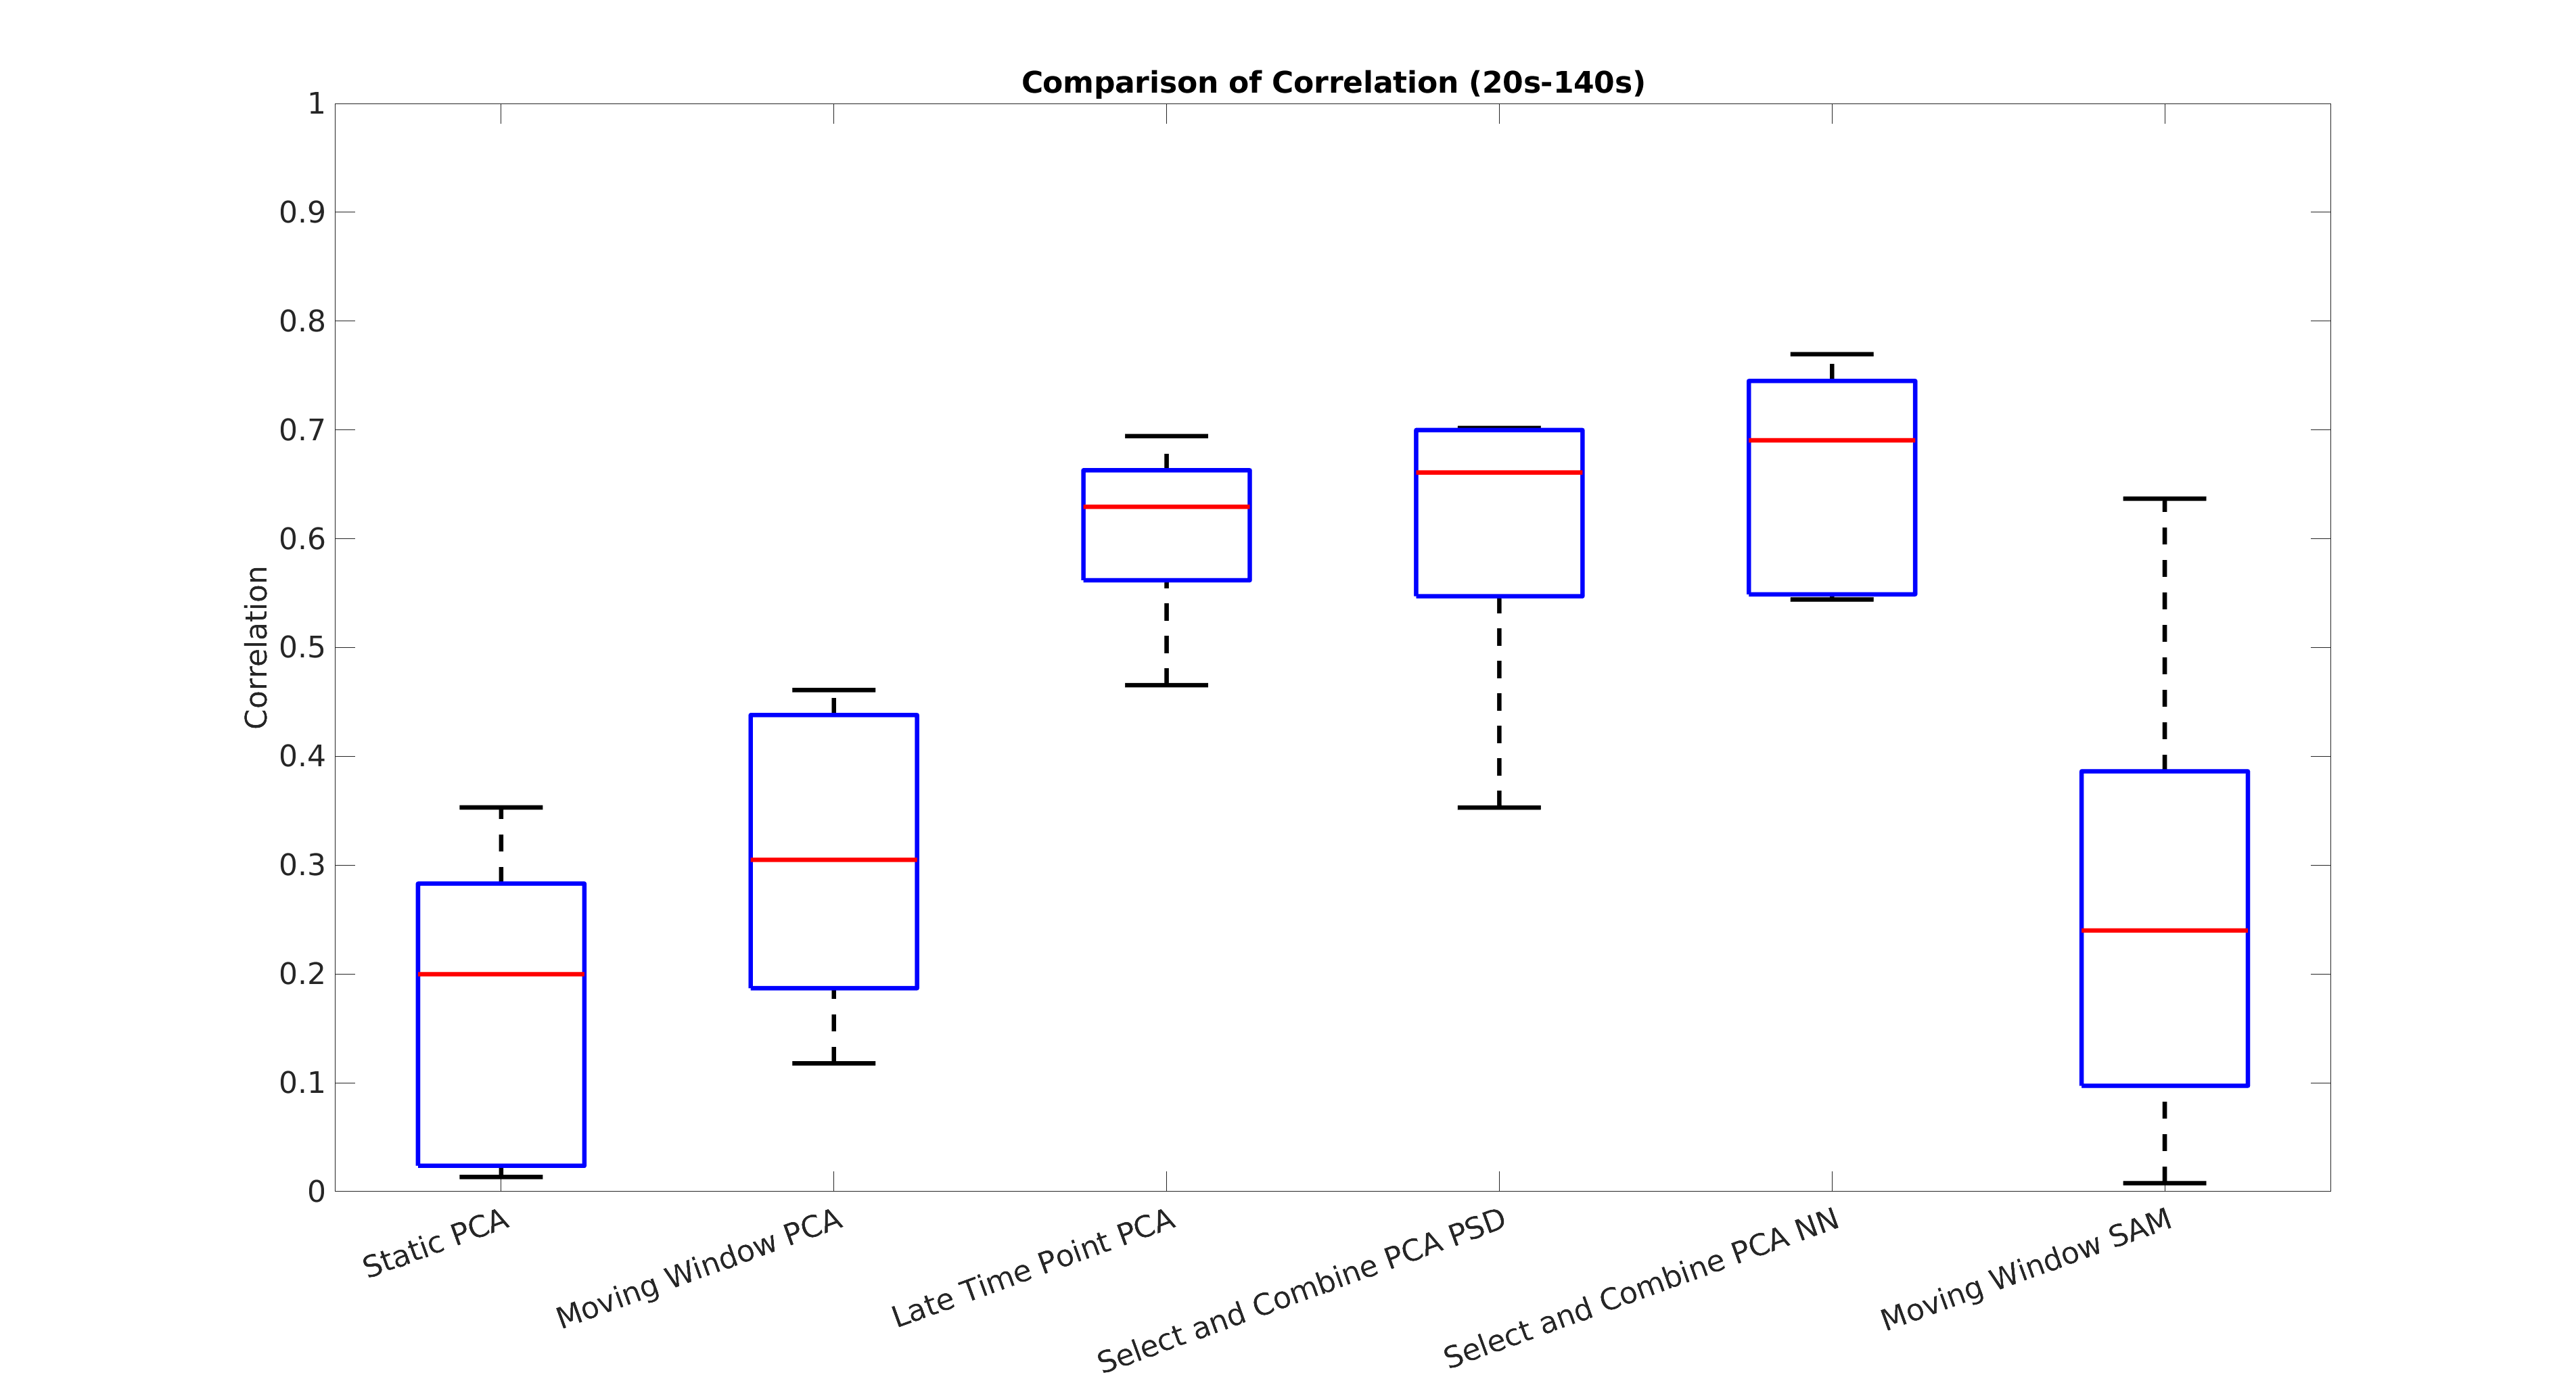
\includegraphics[width=1.0\linewidth]{figures/box_plot_early.png}
        
        % \vspace{-0.4cm}
        
        \captionsetup{singlelinecheck=false, justification=centering}
        \caption{
        % \scriptsize
        A box plot showing for each method its correlation coefficient, to the \gls{RPM}, for the entire acquisition (taken for seven acquisitions).}
        
        \label{fig:box_plot_early}
        
        % % \vspace{-0.5cm}
    \end{figure}
    
        \begin{figure}
        % \vspace{-0.5cm}
        
        \centering
        
        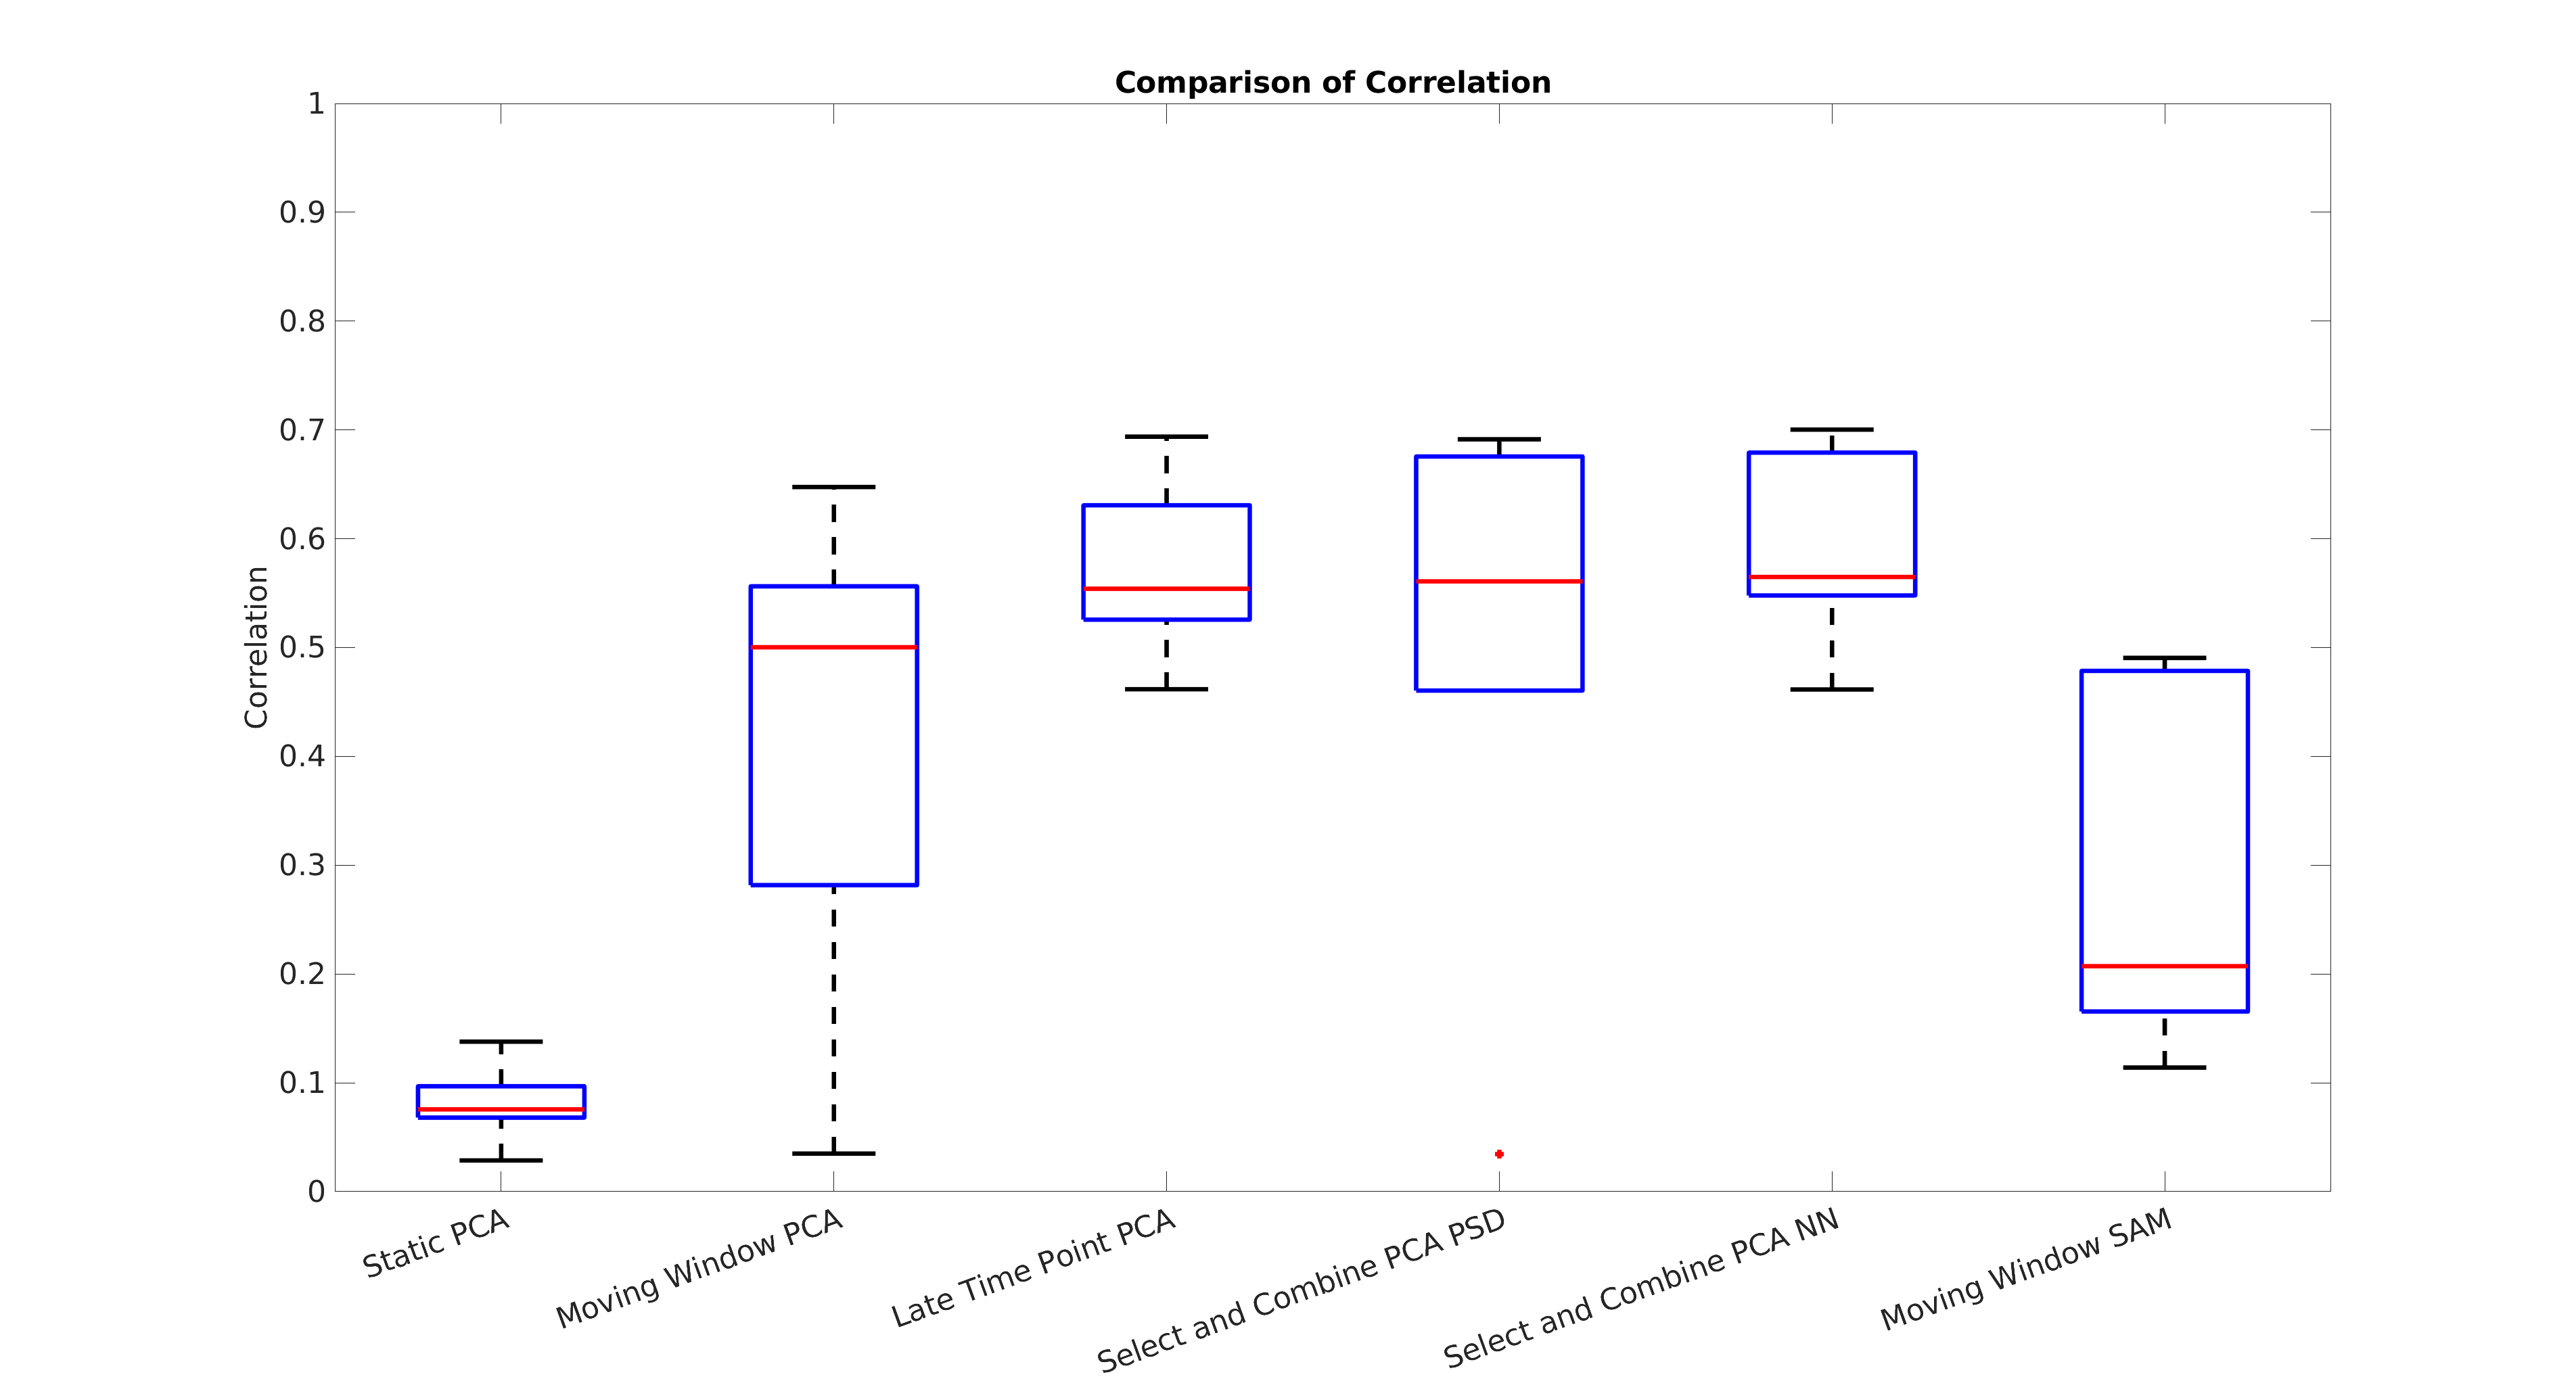
\includegraphics[width=1.0\linewidth]{figures/box_plot_all.png}
        % 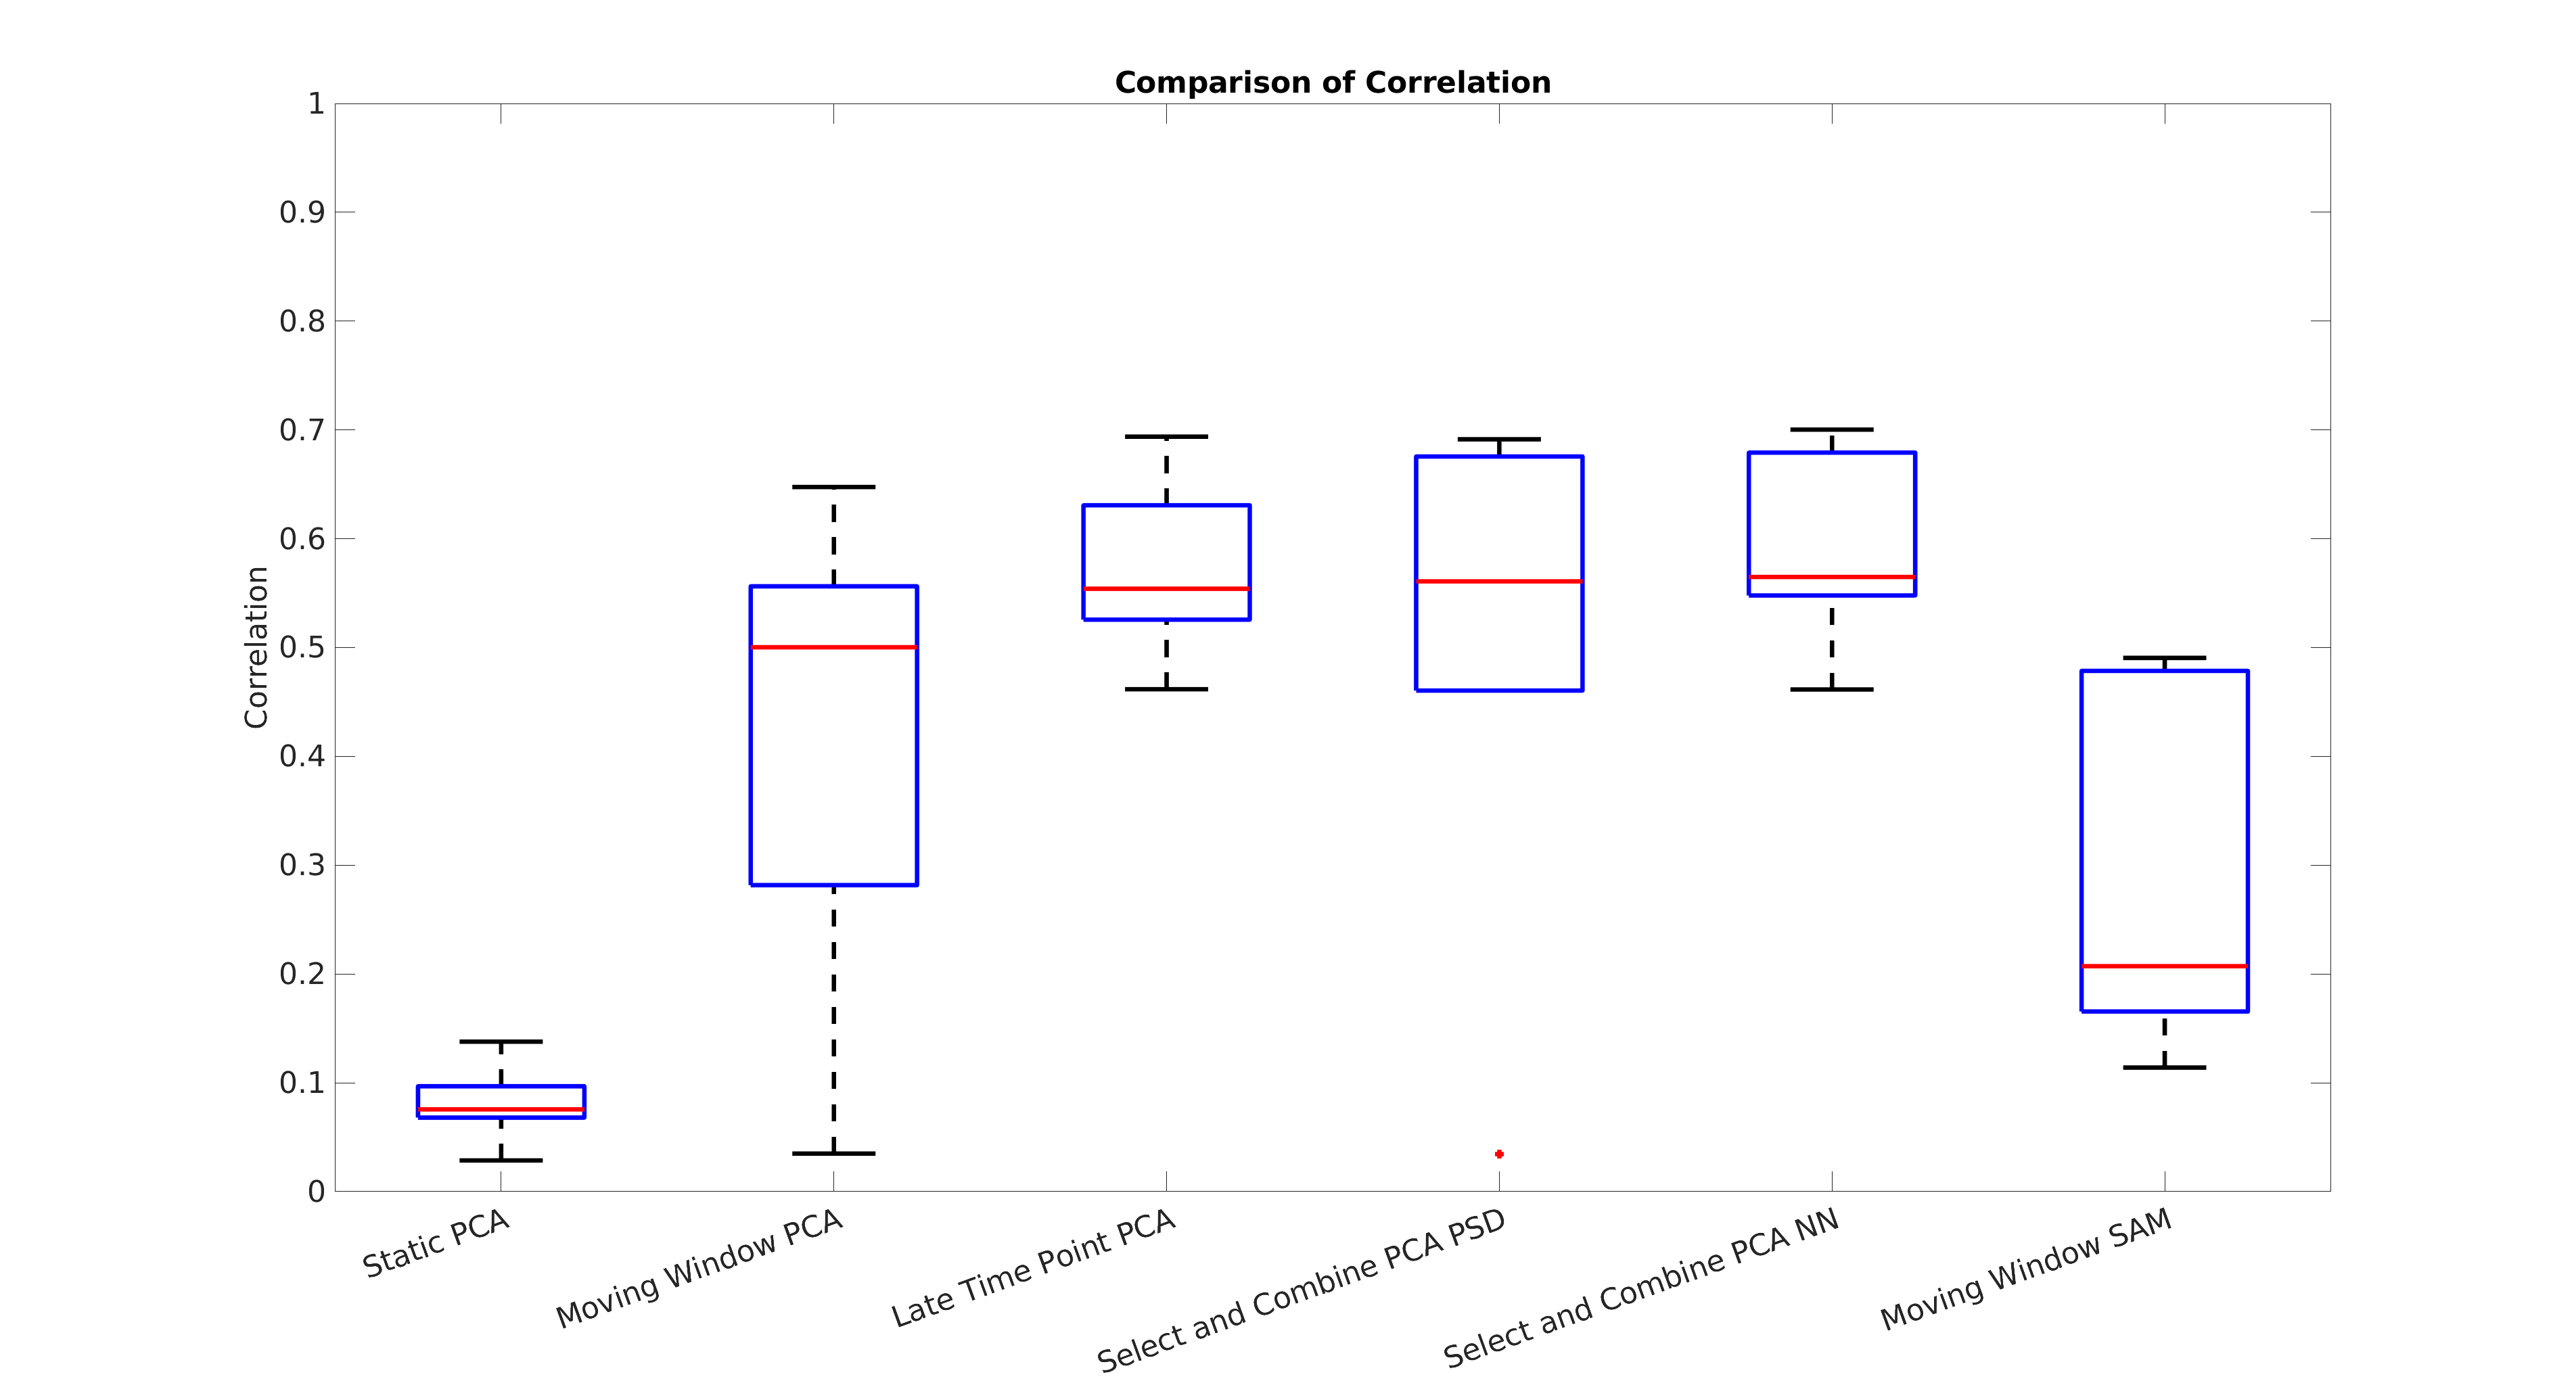
\includegraphics[width=1.0\linewidth]{figures/box_plot_all.png}
        
        % \vspace{-0.4cm}
        
        \captionsetup{singlelinecheck=false, justification=centering}
        \caption{
        % \scriptsize
        A box plot showing for each method its correlation coefficient, to the \gls{RPM}, for the first \SI{120}{\second} (between \SI{20}{\second} and \SI{140}{\second}) (taken for seven acquisitions).}
        
        \label{fig:box_plot_all}
        
        % % \vspace{-0.5cm}
    \end{figure}
    
    % \begin{figure}
        % \vspace{-0.5cm}
        
    %     \centering
        
    %     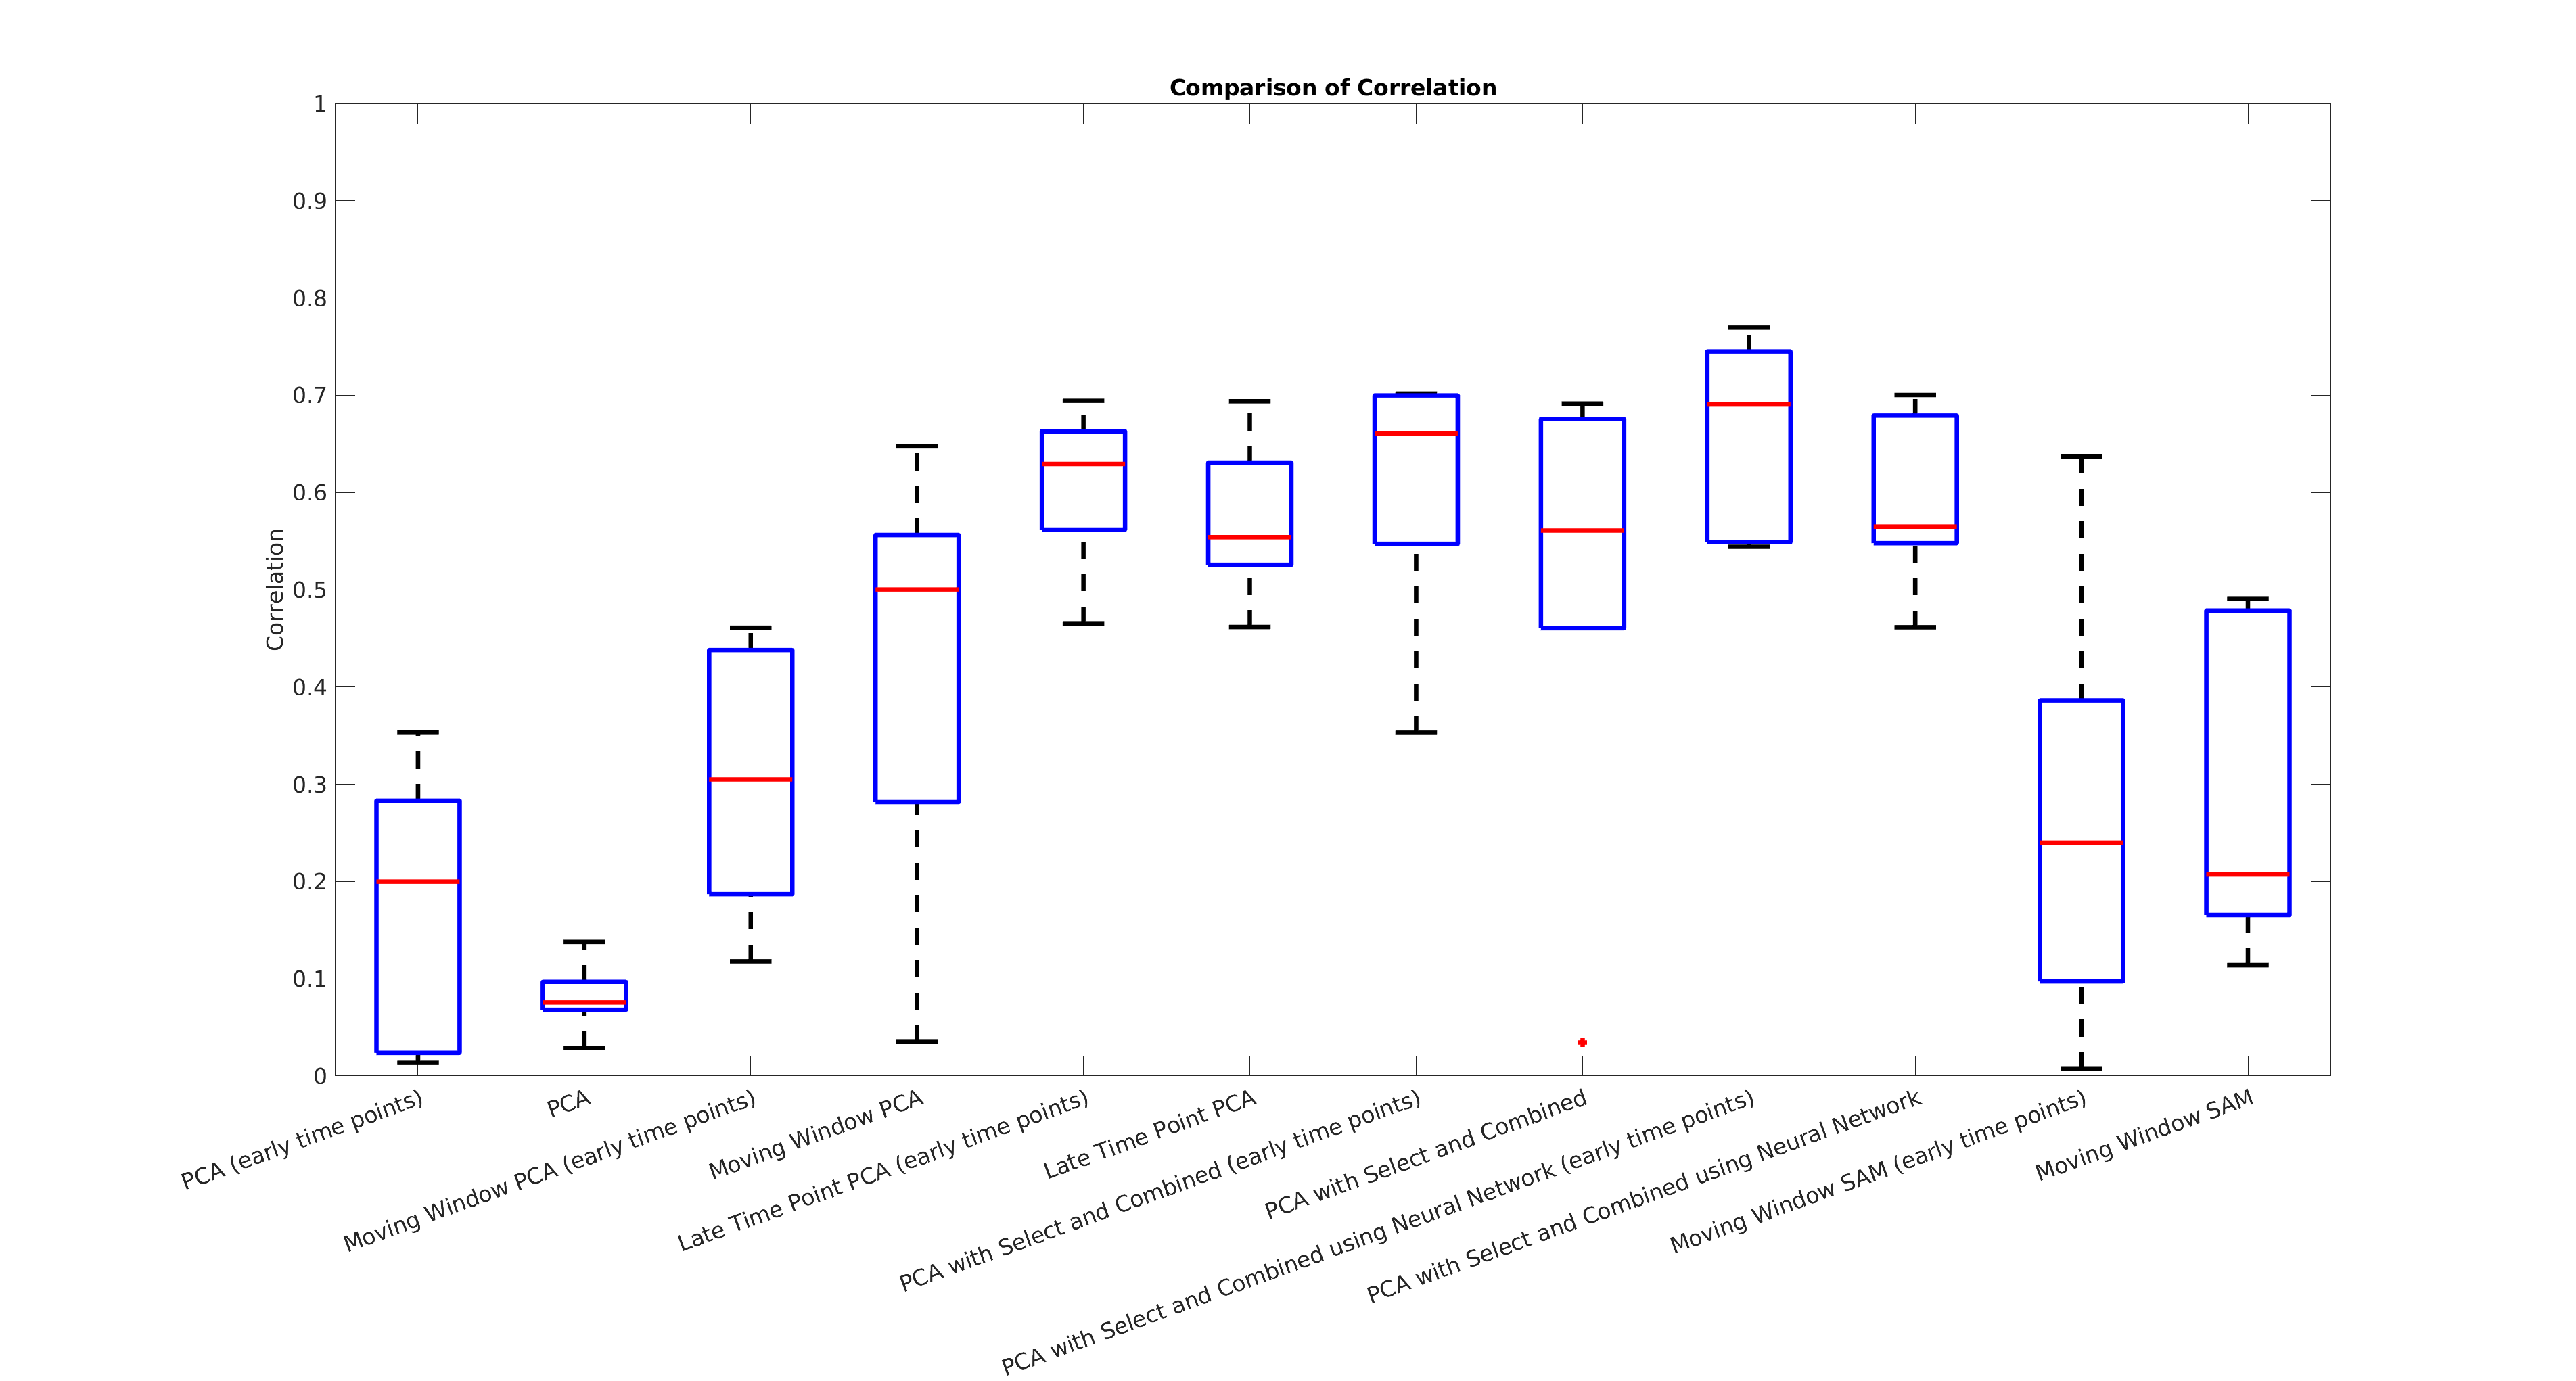
\includegraphics[width=1.0\linewidth]{figures/box_plot.png}
        % 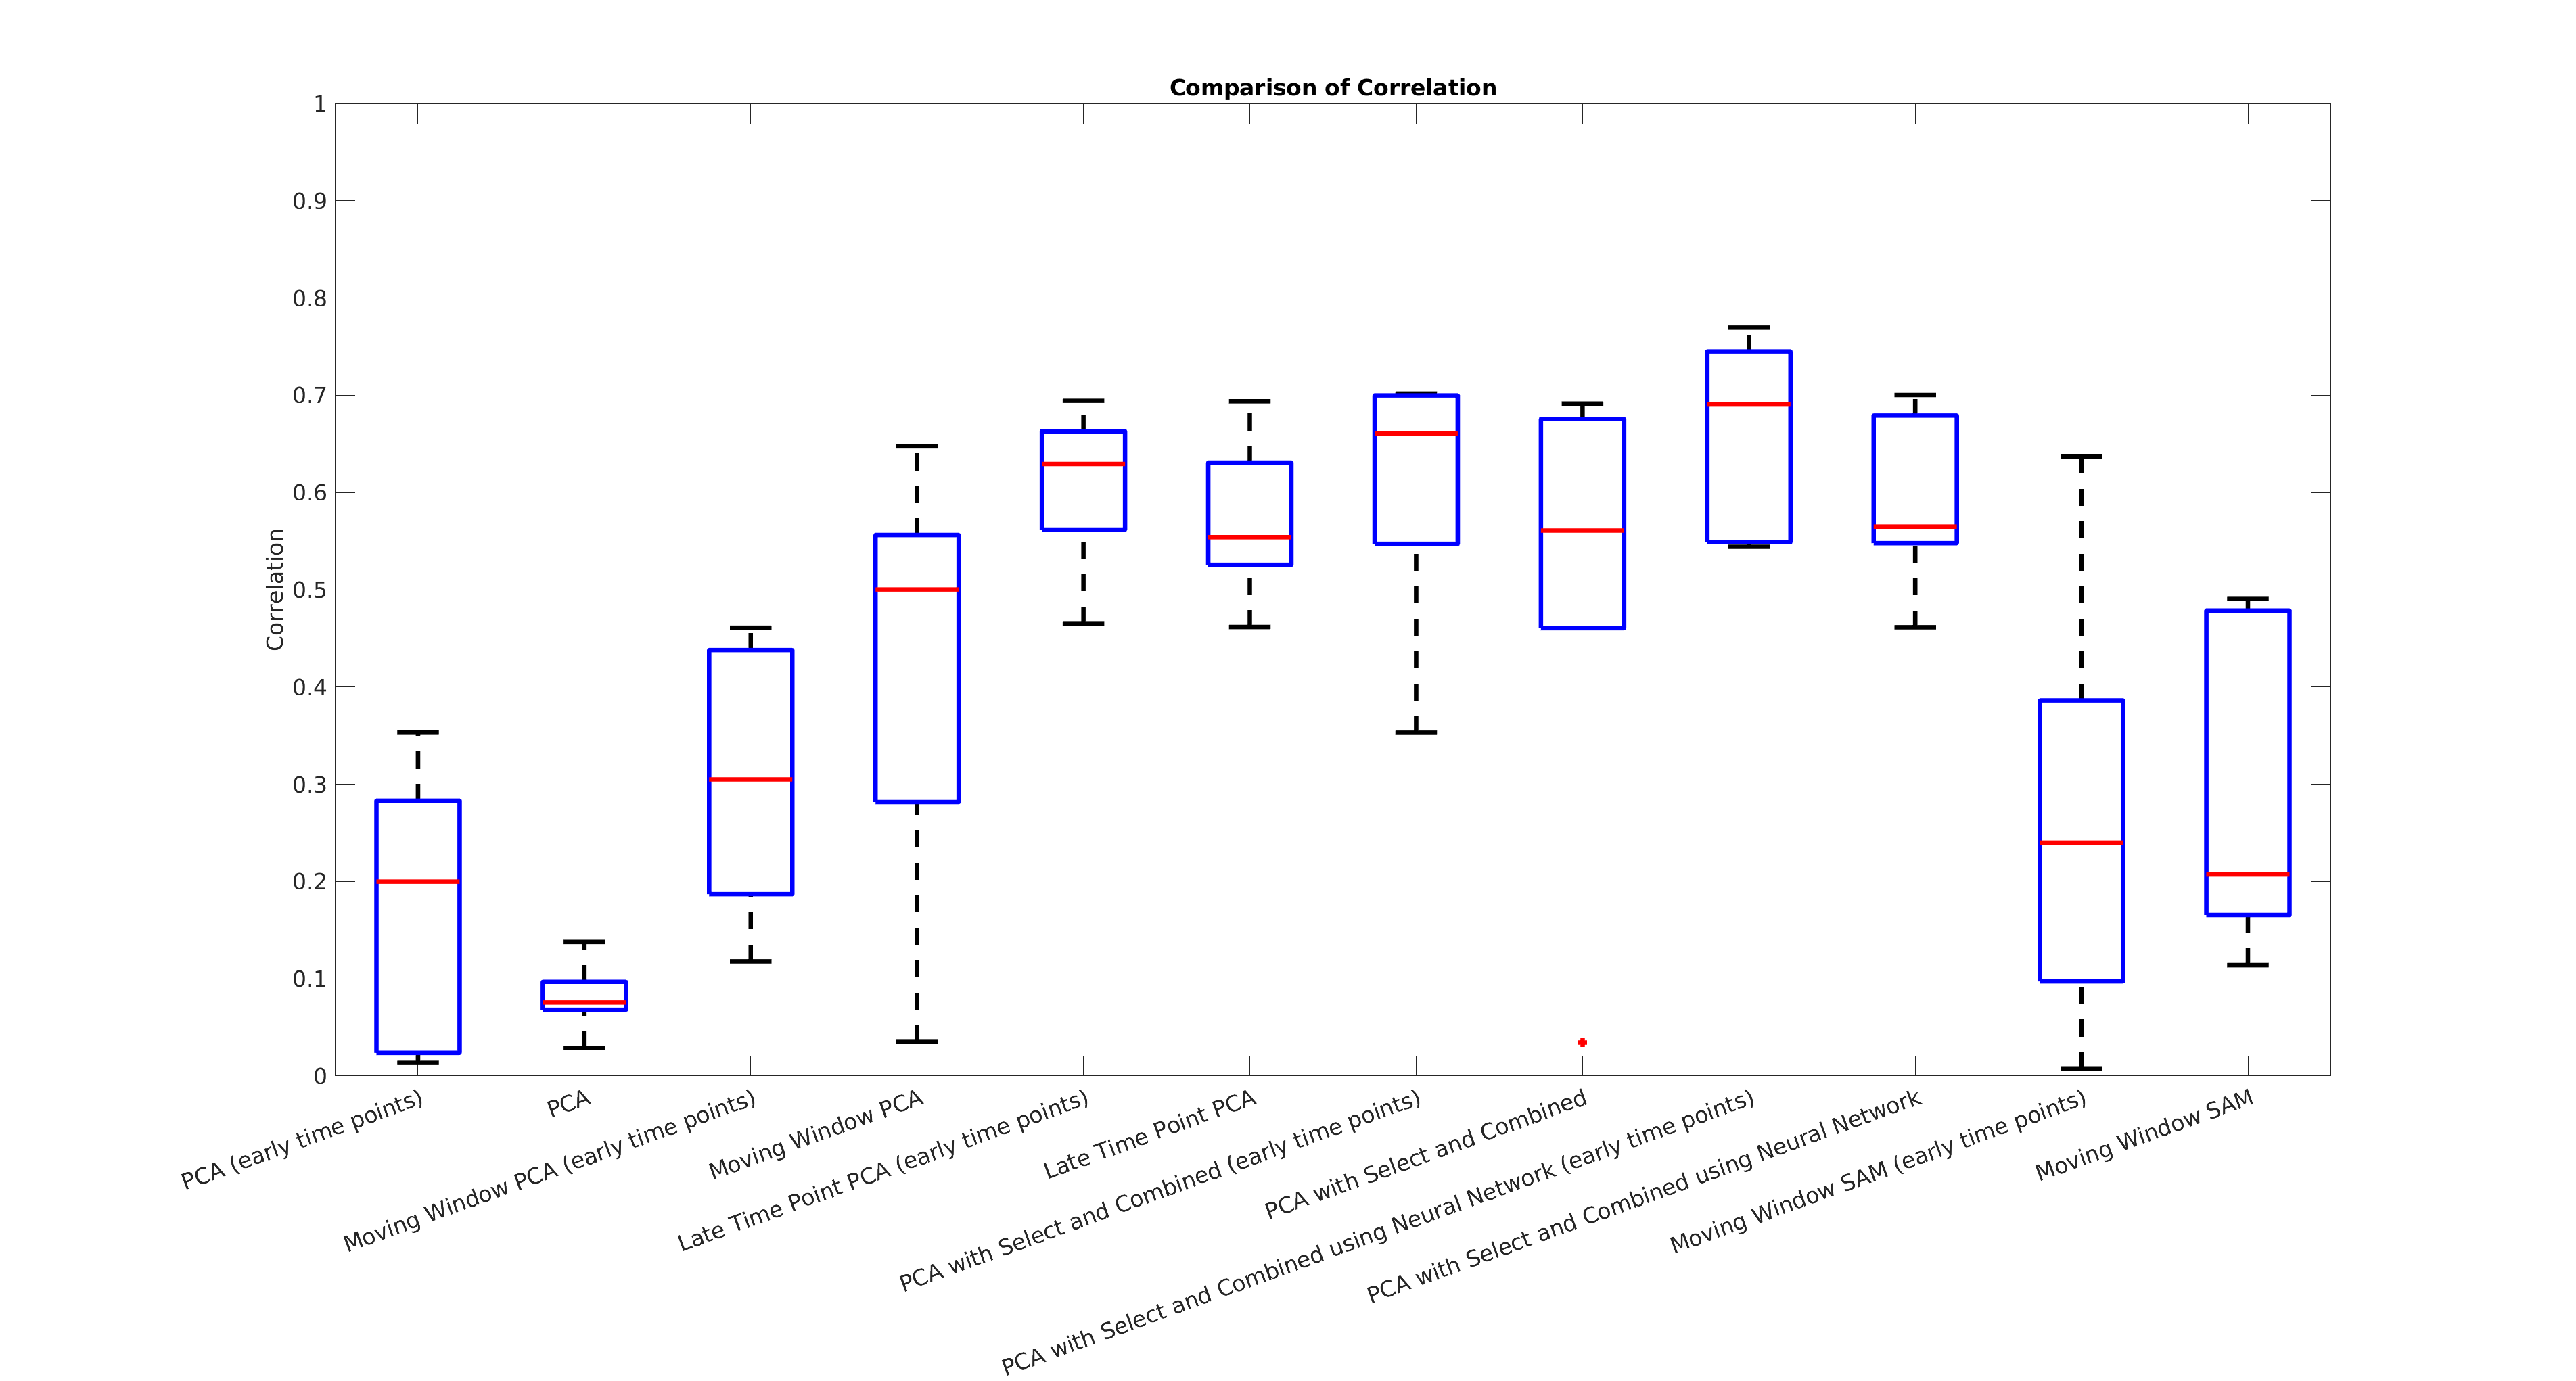
\includegraphics[width=1.0\linewidth]{figures/box_plot.png}
        
        % \vspace{-0.4cm}
        
    %     \captionsetup{singlelinecheck=false, justification=centering}
    %     \caption{
        % \scriptsize
    %     A box plot showing for each method its correlation coefficient, to the \gls{RPM}, for both the first \SI{120}{\second} (between \SI{20}{\second} and \SI{140}{\second}), and also for the entire acquisition (taken for seven acquisitions).}
        
    %     \label{fig:box_plot}
        
        % % \vspace{-0.5cm}
    % \end{figure}
    
    \begin{figure}
        % % \vspace{-0.5cm}
        
        \centering
        
        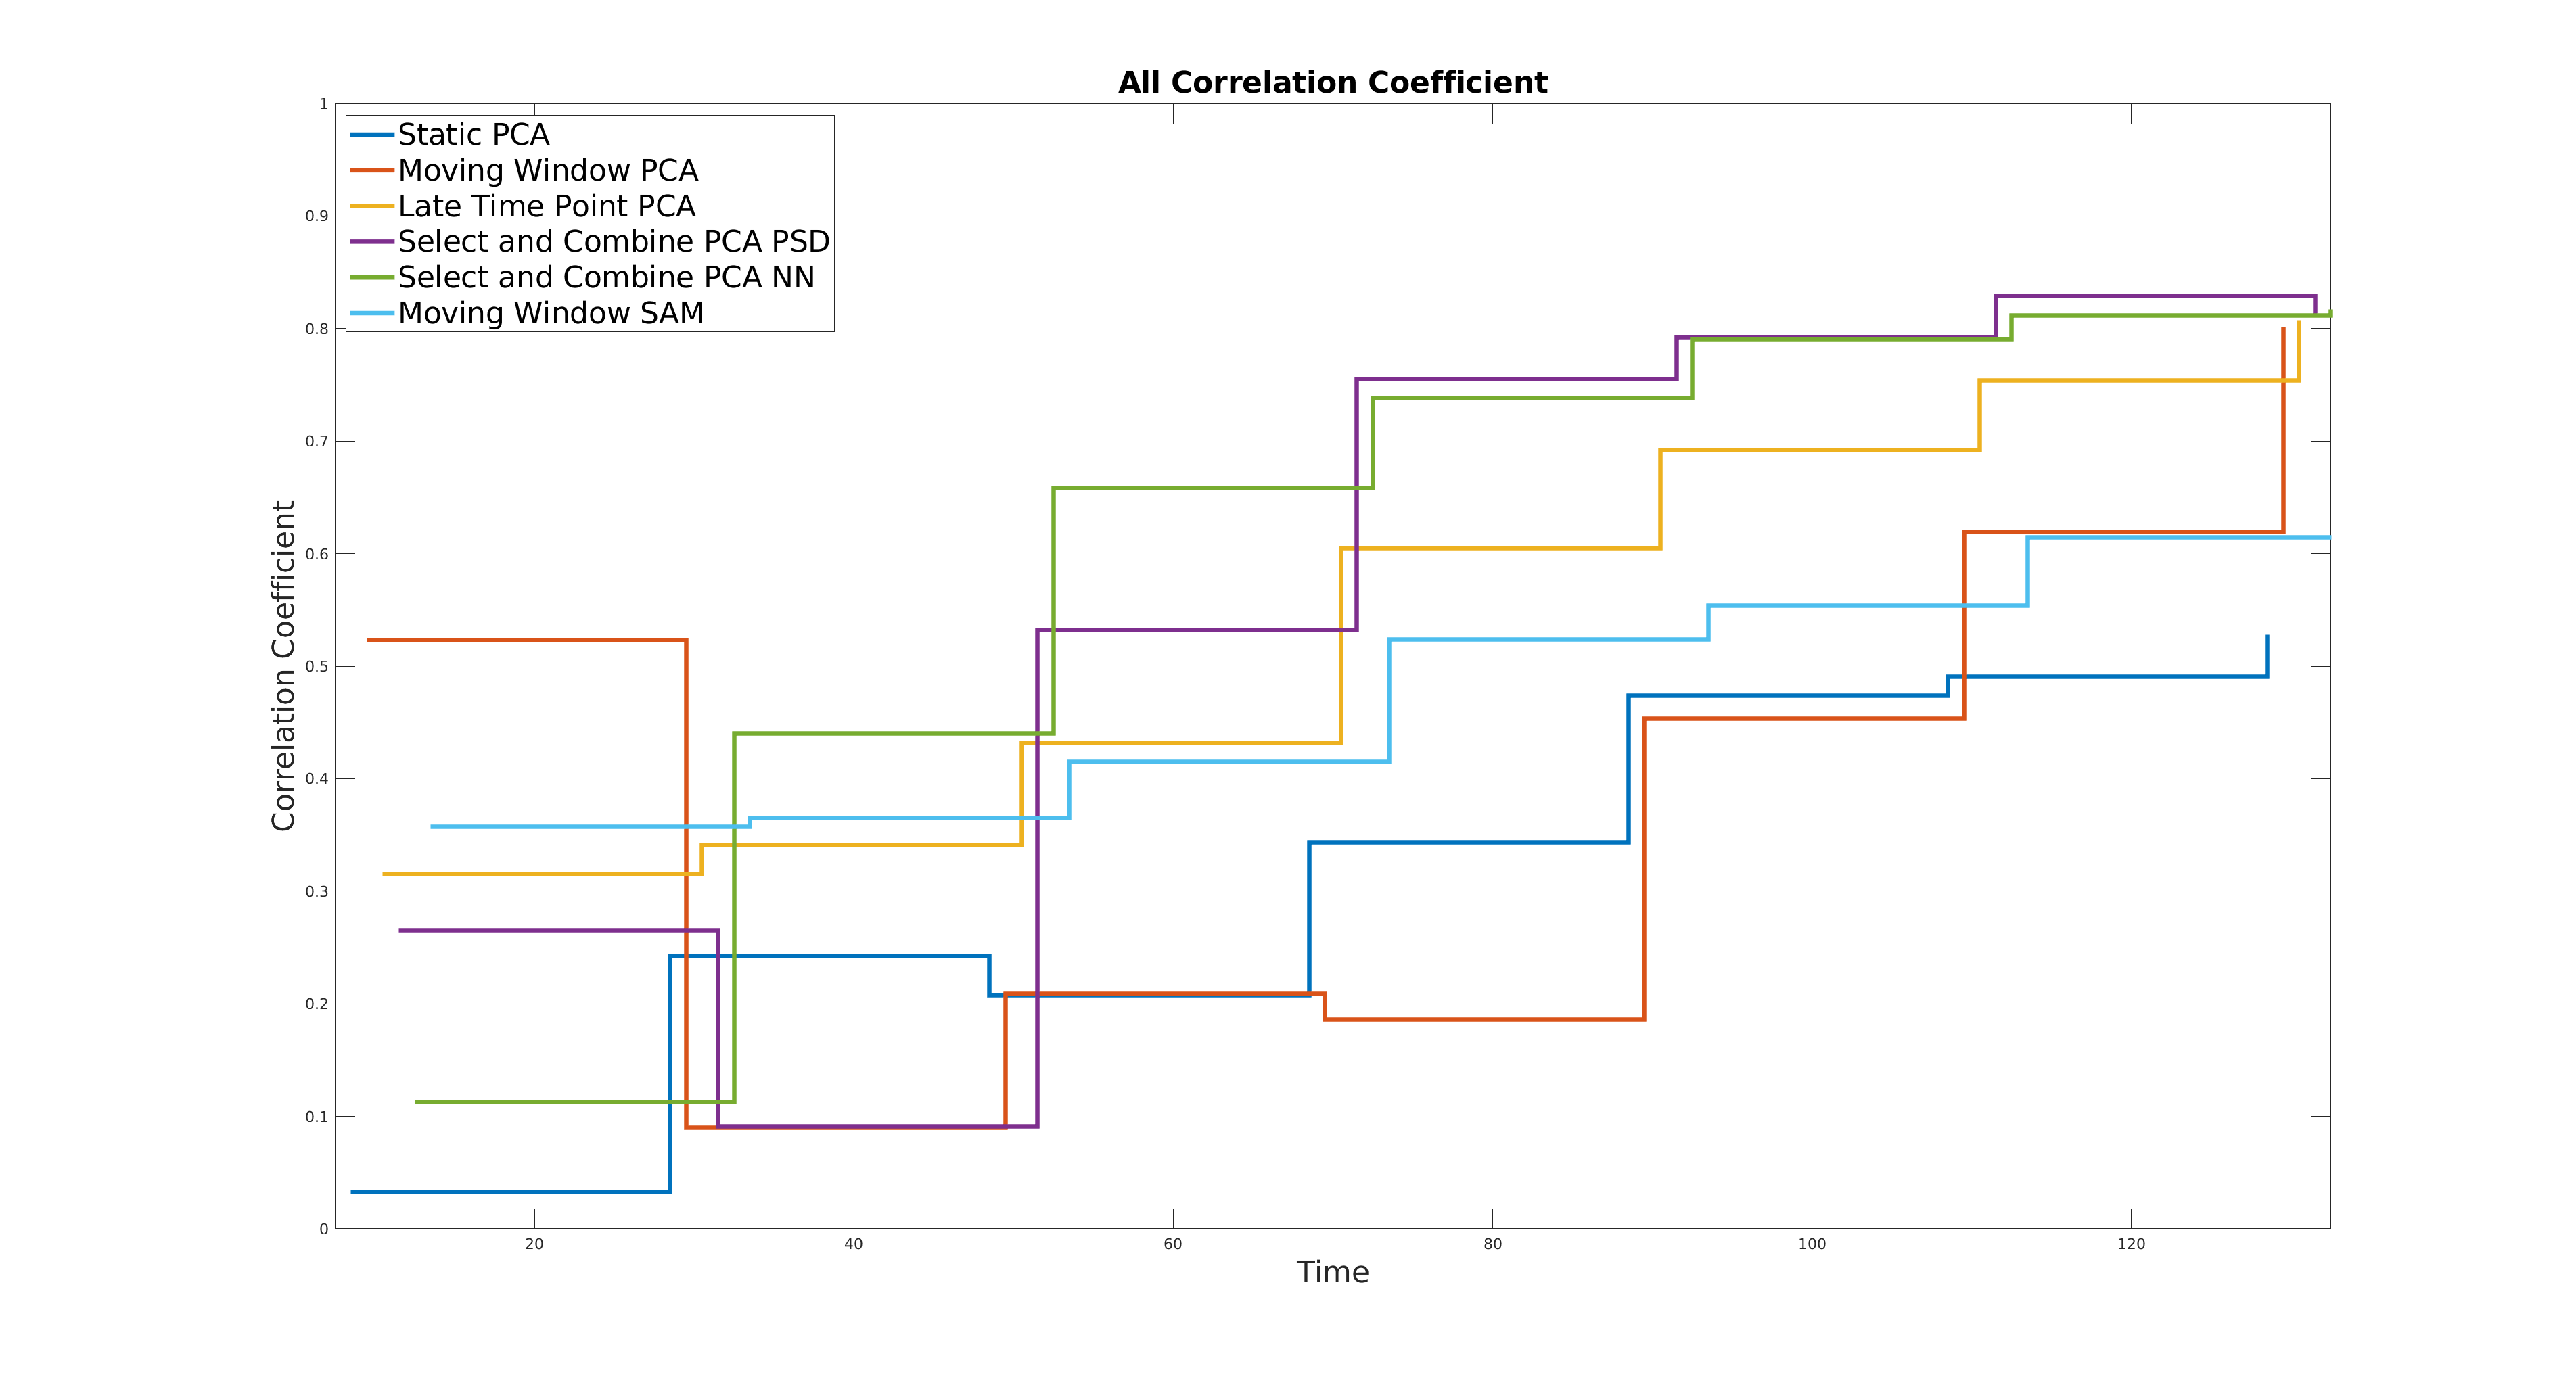
\includegraphics[width=1.0\linewidth]{figures/all_correlation_coefficient.png}
        % 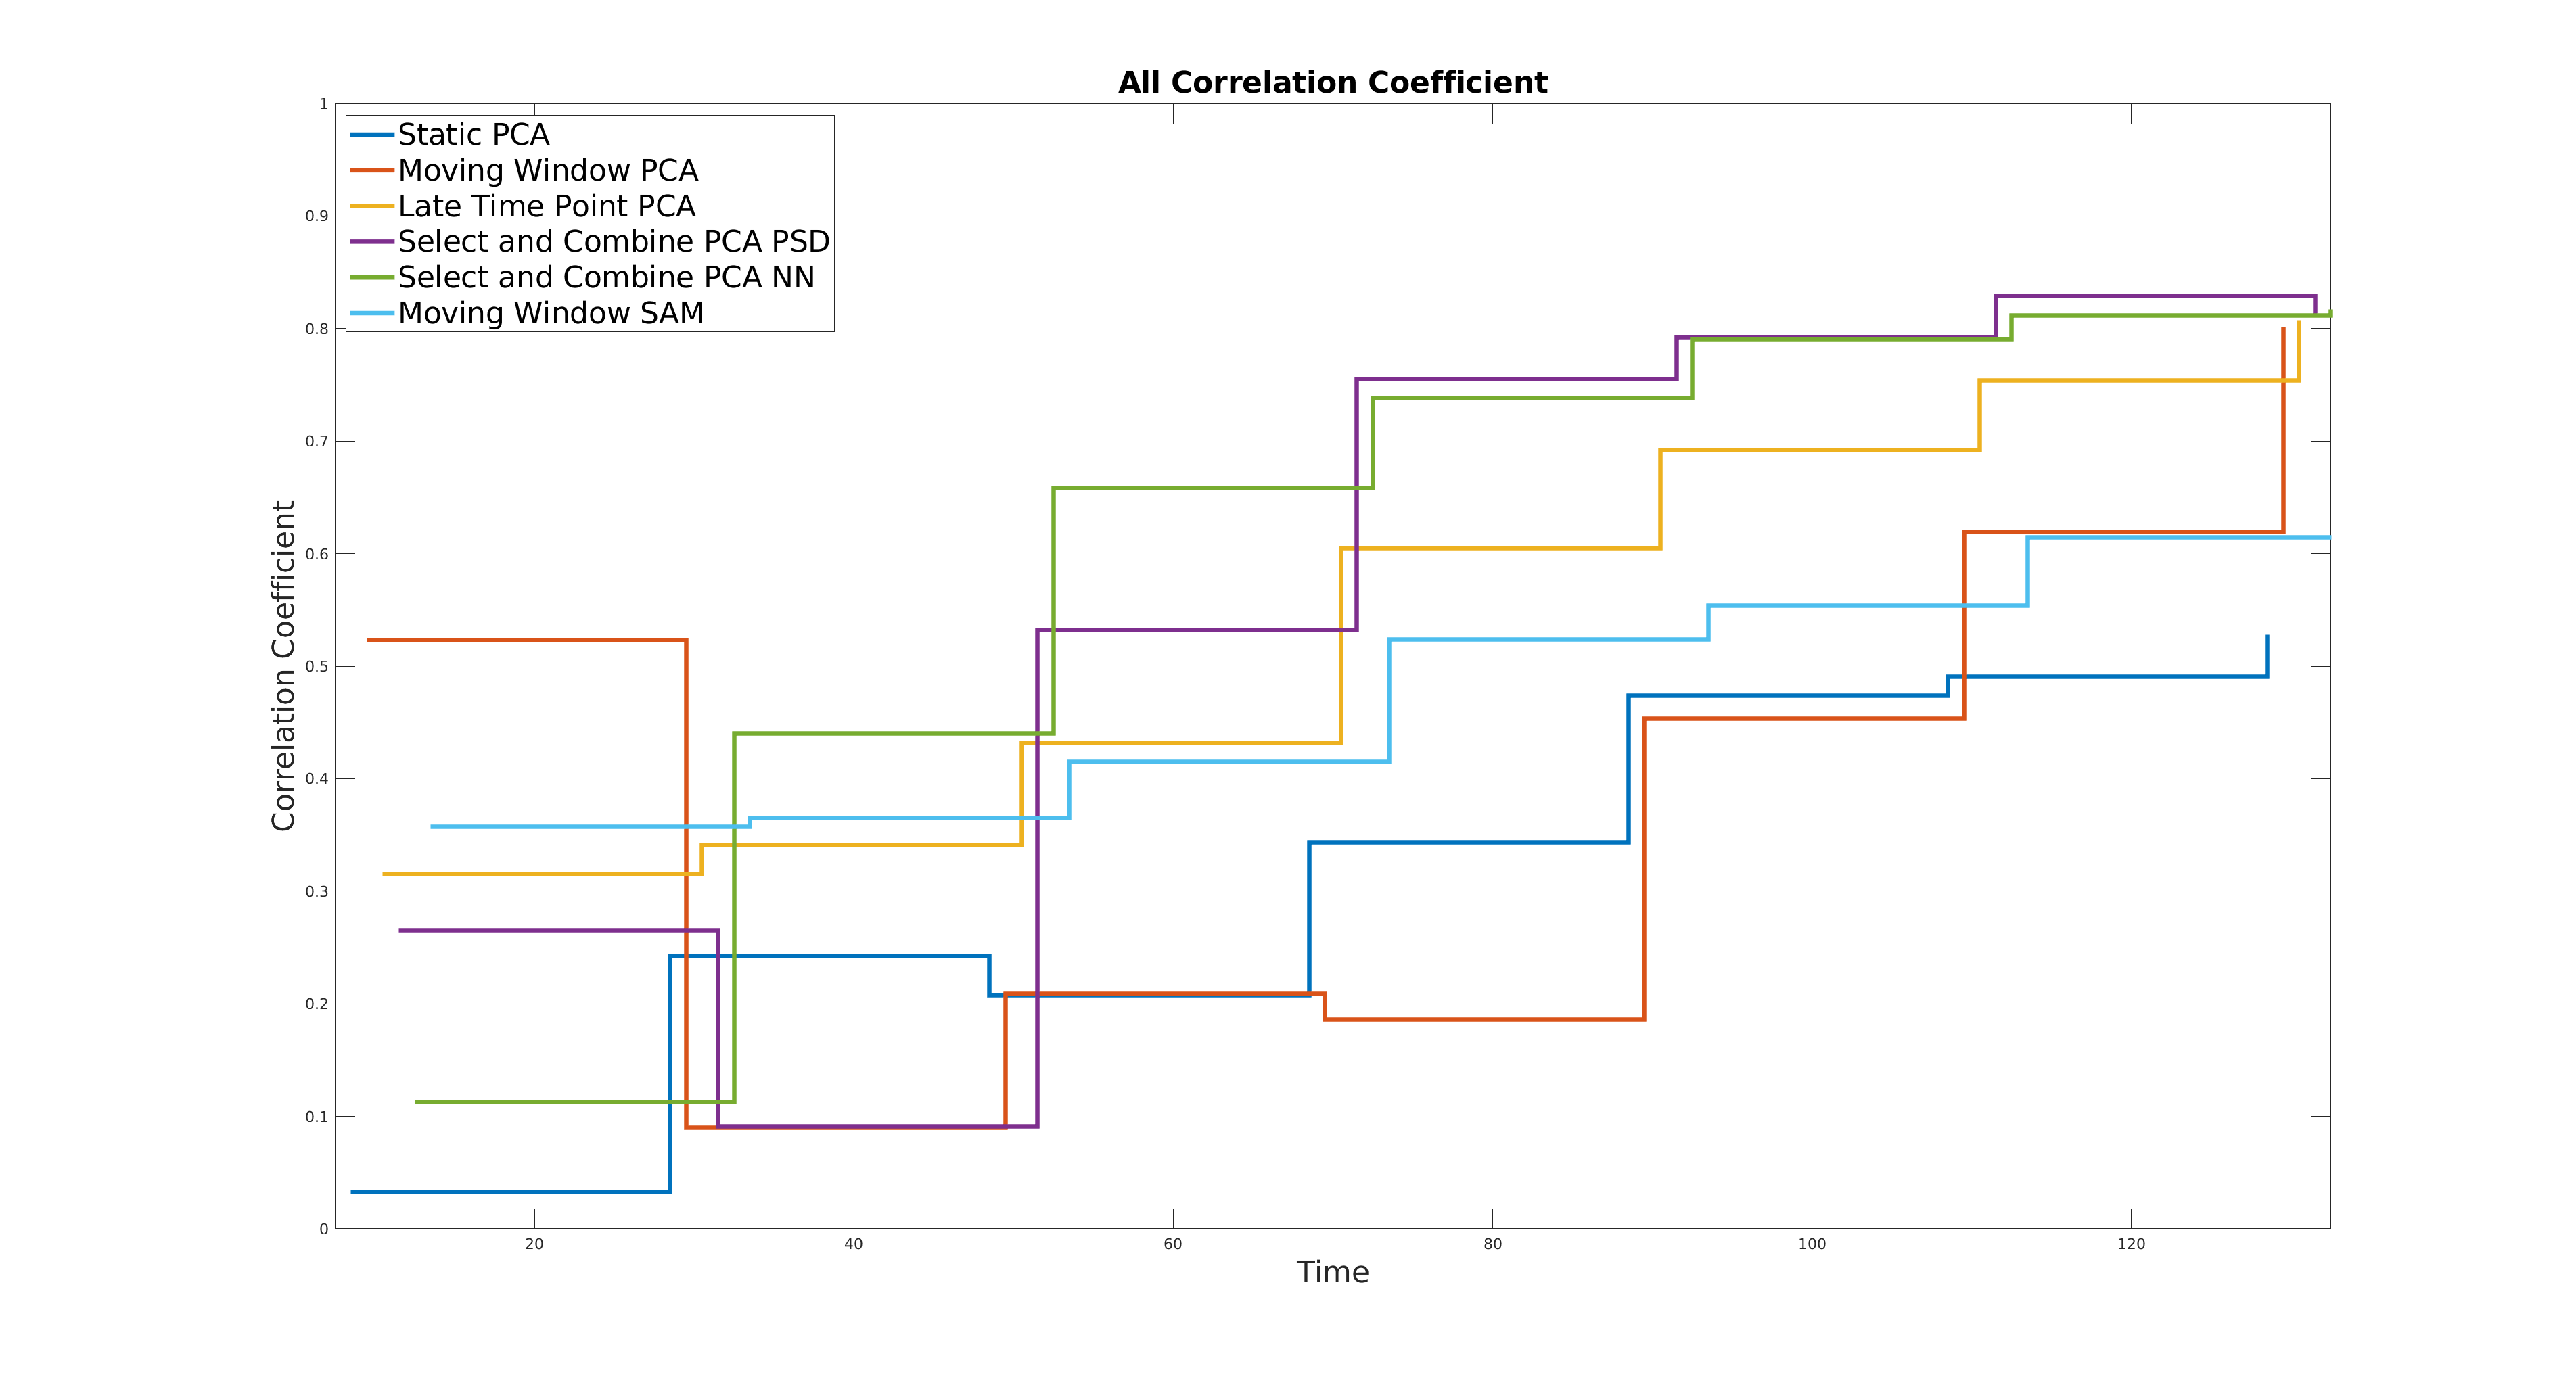
\includegraphics[width=1.0\linewidth]{figures/all_correlation_coefficient.png}
        
        % \vspace{-0.5cm}
        
        \captionsetup{singlelinecheck=false, justification=centering}
        \caption{
        % \scriptsize
        A plot showing for each method its correlation coefficient, to the \gls{RPM}, for the first \SI{120}{\second} (between \SI{10}{\second} and \SI{130}{\second}, in \SI{20}{\second} windows, taken as a mean for all data).}
        
        \label{fig:all_cross_correlation}
        
        % \vspace{-0.5cm}
    \end{figure}
    
    \begin{figure}
        % \vspace{-0.5cm}
        \centering
    
        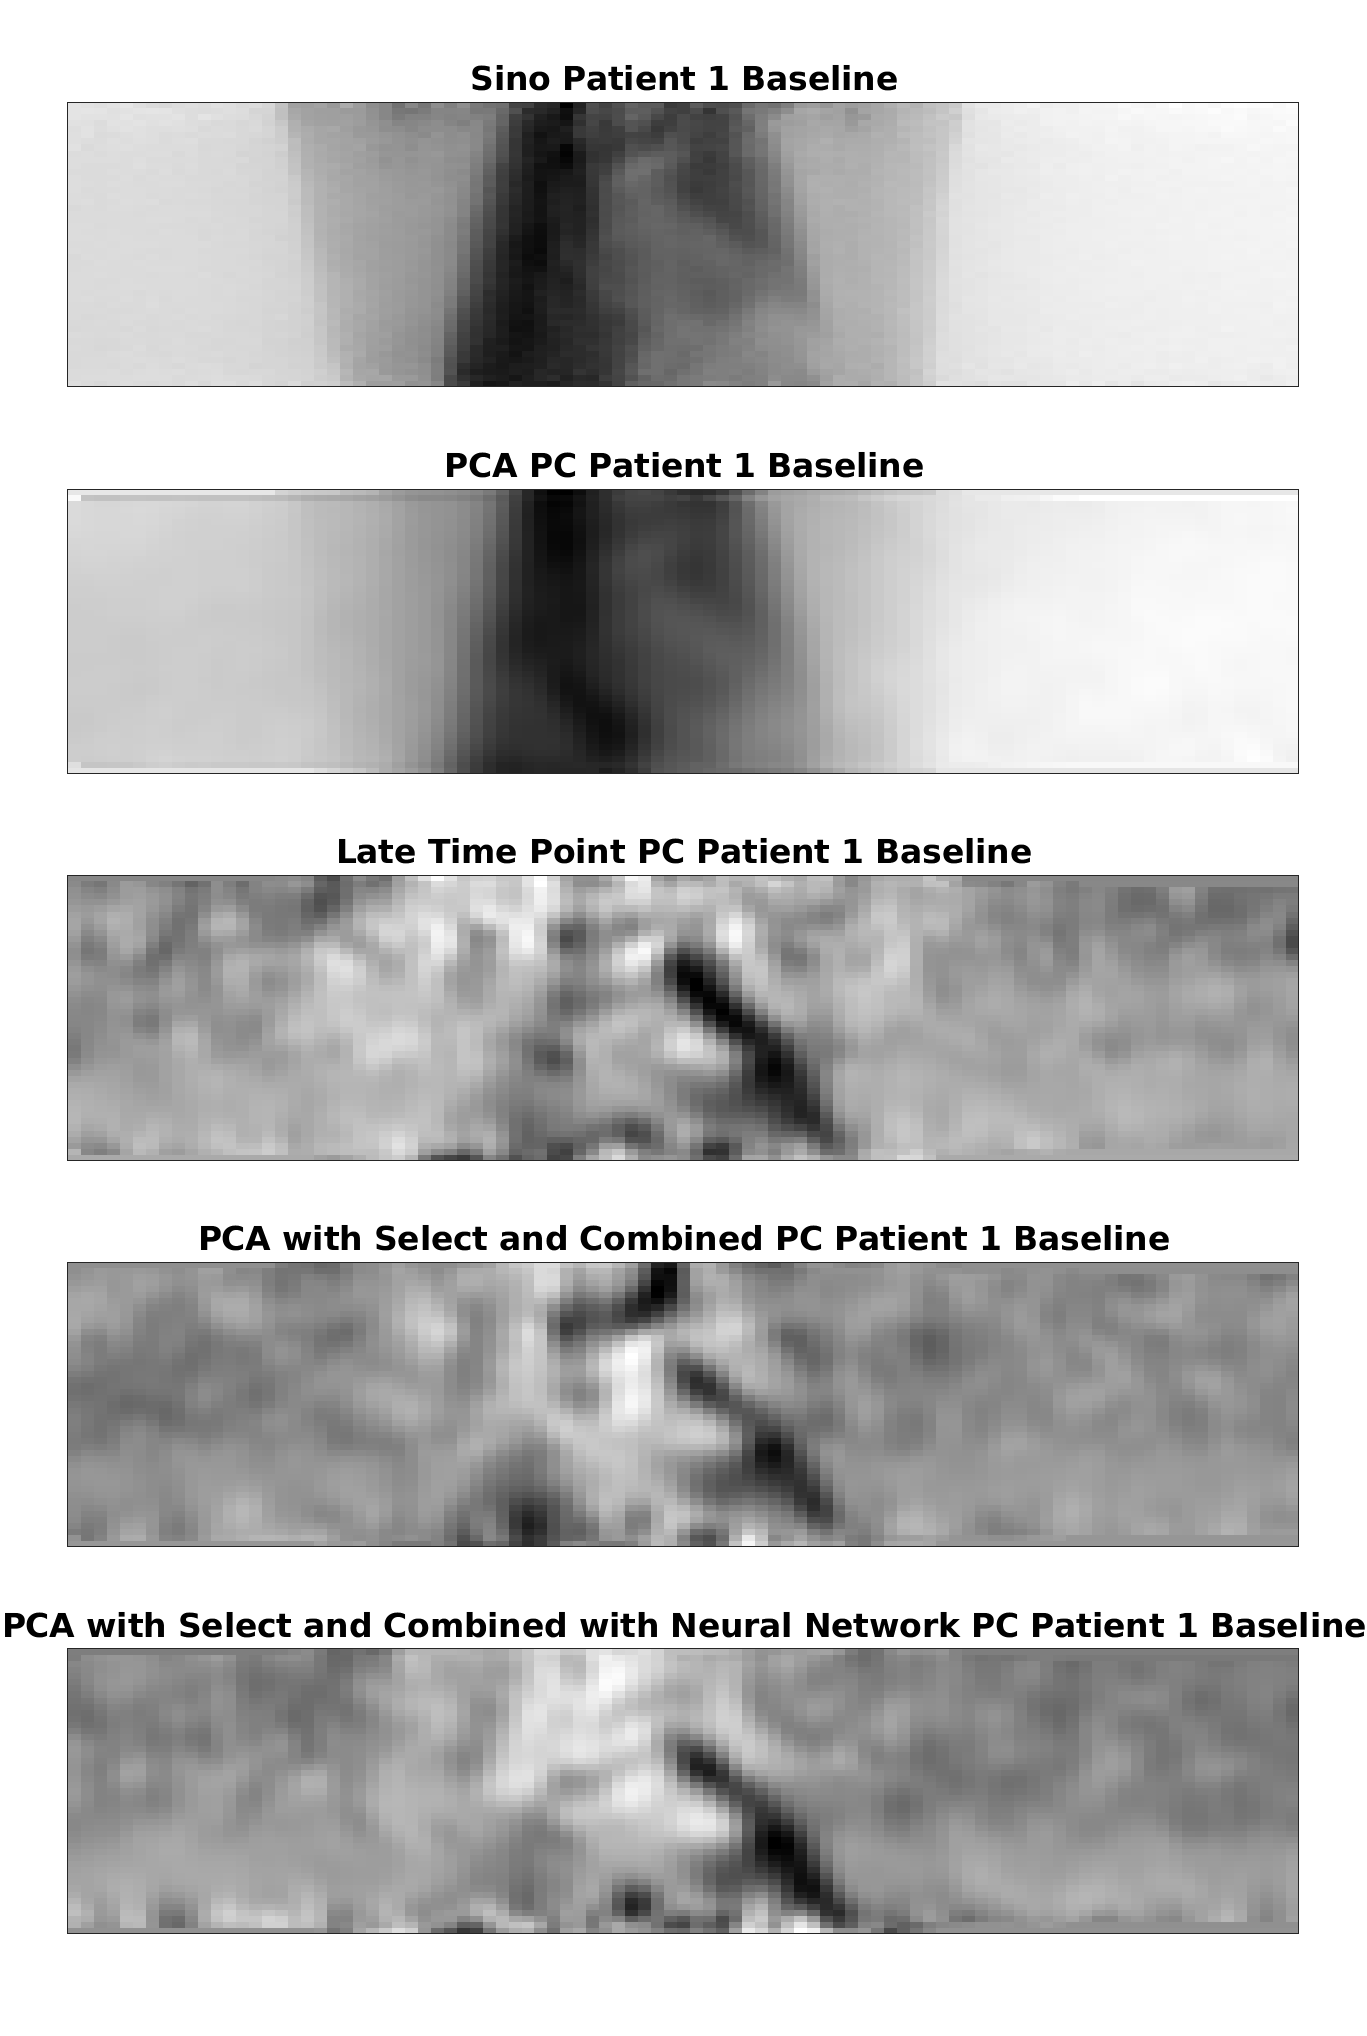
\includegraphics[width=1.0\linewidth]{figures/patient_one_pc_output.png}    
        % 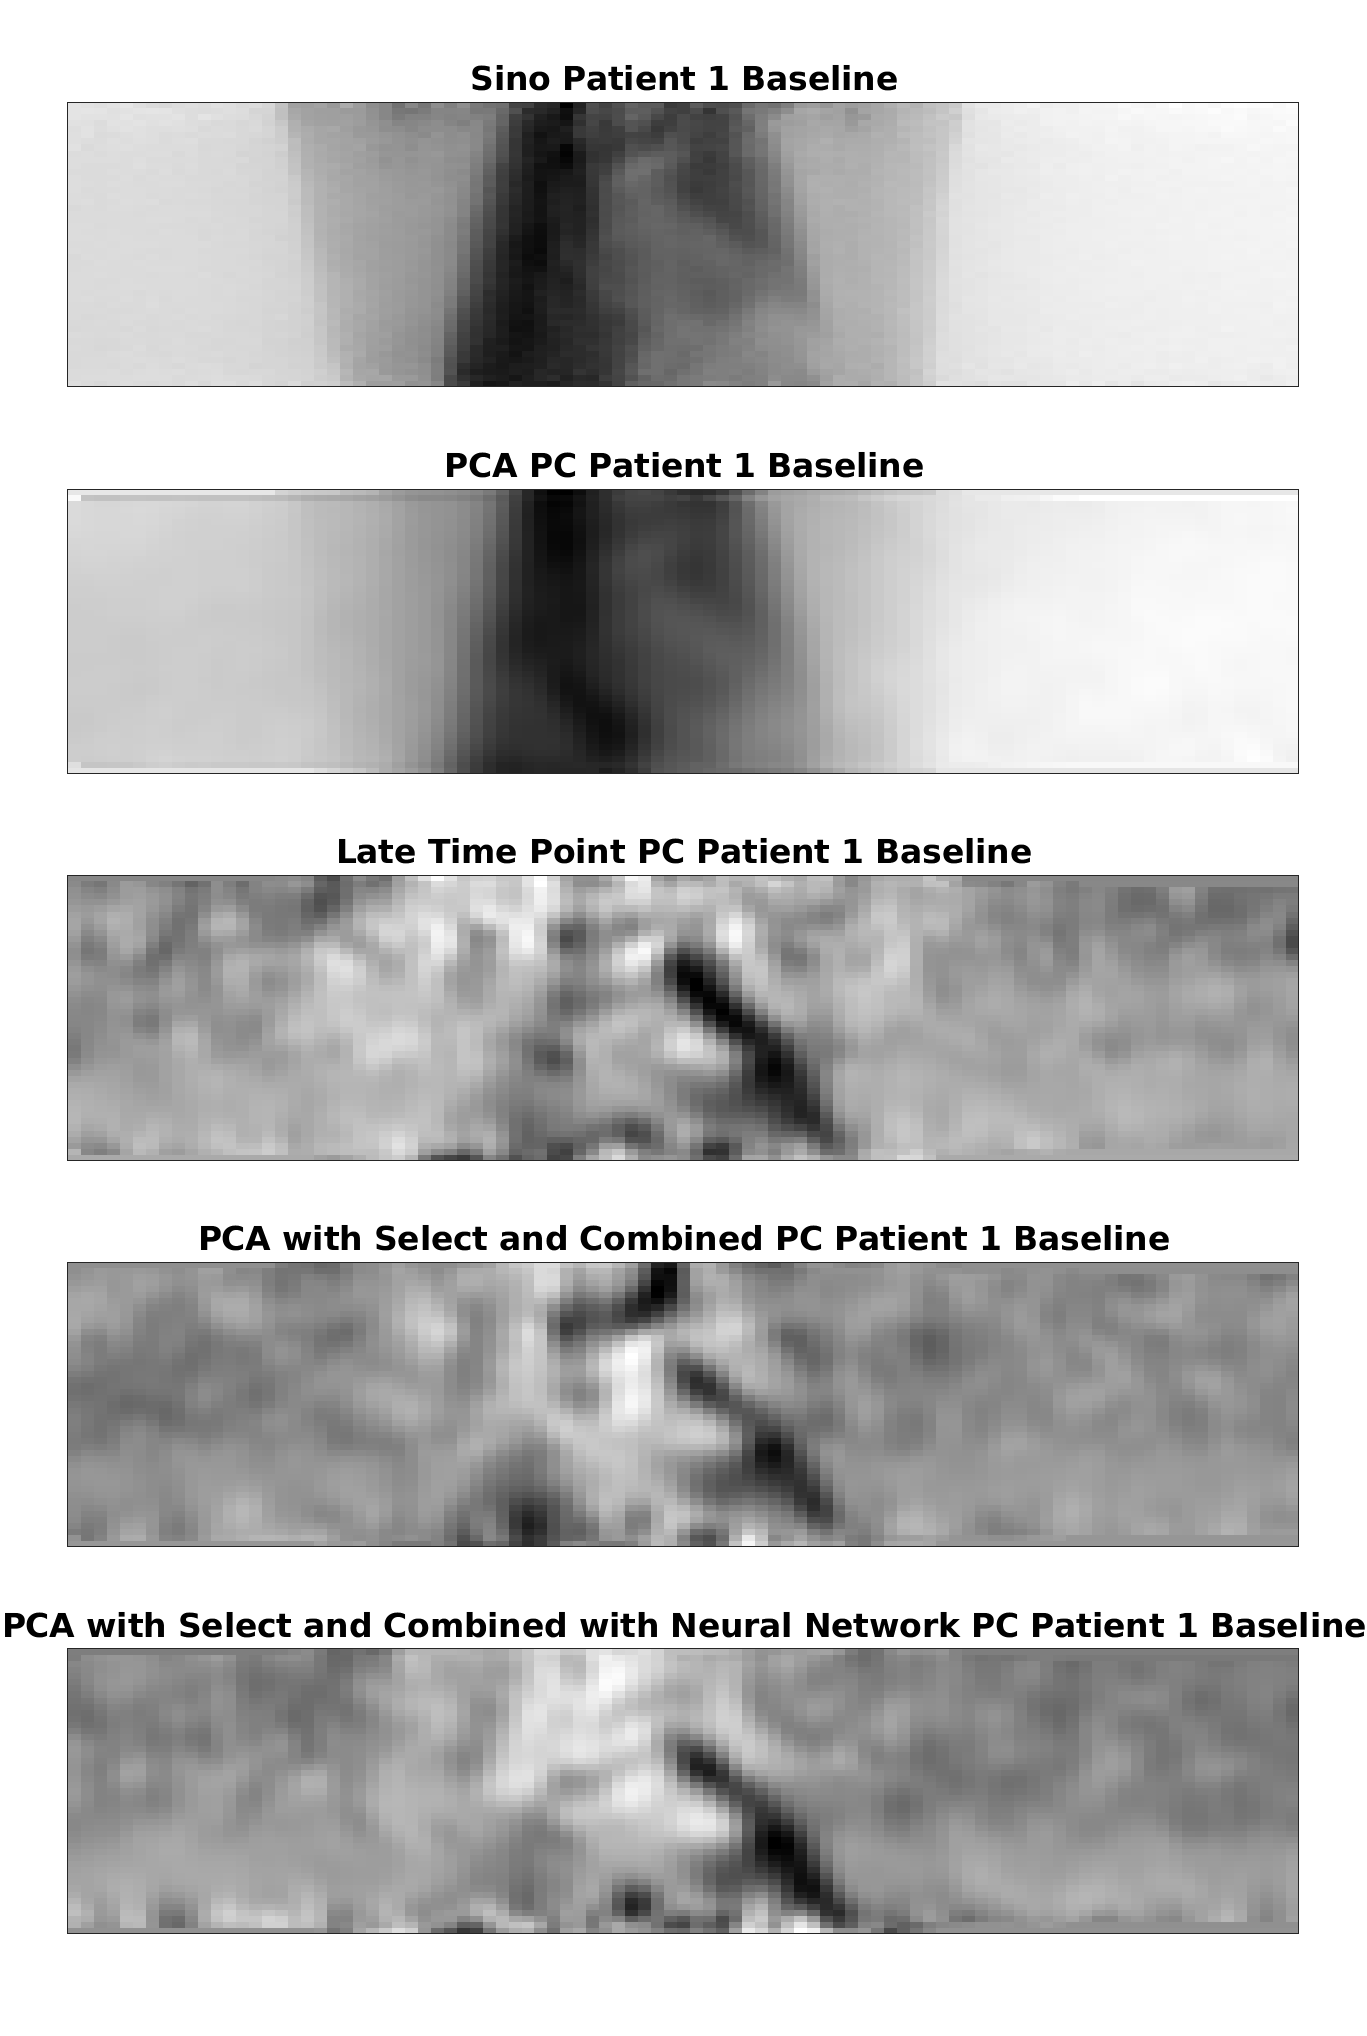
\includegraphics[width=1.0\linewidth]{figures/patient_one_pc_output.png}
    
        % \vspace{-0.5cm}
        
        \captionsetup{singlelinecheck=false, justification=centering}
        \caption{
        % \scriptsize
        A plot showing the \gls{PC} used to generate the output signal (taken for the first acquisition of patient one).}
    
        \label{fig:patient_one_pc_output}
    
        % \vspace{-0.5cm}
    \end{figure}
    
    From~\Fref{fig:patient_one_output} and~\Fref{fig:all_cross_correlation} it can be observed that the Static \acrshort{PCA} method has failed, as expected. Both Moving Window methods extract a signal at later time points only. The Late Time Point, Select and Combine \gls{PSD}, and Select and Combine \gls{NN} methods all appear to be able to extract a usable signal, down to \SI{20}{\second} after the start of the scan.
    
    In~\Fref{fig:box_plot_early} and~\Fref{fig:box_plot_all}, the improvement of the Late Time Point, Select and Combine \gls{PSD}, and Select and Combine \gls{NN} methods is most apparent, with high correlation coefficients for both the early time point, as well as for all data. The Select and Combine methods show marginally higher correlation coefficients than the Late Time Point method, and the \gls{NN} shows slightly higher correlation coefficients than the \gls{PSD}.
    
    In~\Fref{fig:patient_one_pc_output} it can be observed the Static \acrshort{PCA} method returns a \gls{PC} which closely resembles the input data, leading to the conclusion that variation from a number of sources is included. It appears from a visual inspection that the least confounding variation and noise is included in the Select and Combine with \gls{NN} method.

% \vspace{-0.4cm}

\section{DISCUSSION AND CONCLUSIONS} \label{sec:discussion_and_conclusions}
    Results from the comparison to the \gls{RPM} indicate, the Late Time Point and both Select and Combine methods are more robust and afford higher quality signals than both Moving Window methods. The results also indicate, both Select and Combine methods can give a higher correlation coefficient earlier than the Late Time Point method. The \gls{NN} shows slightly higher correlation coefficient than the \gls{PSD}.
    
    In the future, research will focus on further development of the method, including, optimisation of the \gls{NN} scoring method. In the next stage, these methods will be applied to the task of implementing advanced respiratory \acrlong{MC} on dynamic \acrshort{PET} data.

\AtNextBibliography{\small}
\printbibliography

\end{document}
